\documentclass[12pt,a4paper]{article}
\usepackage[utf8]{inputenc}

\usepackage{a4wide}

\newcommand{\FIMUreport}[5]{%
{
% Page layout -- do not change!!!
\renewcommand{\baselinestretch}{1.24}
\addtolength{\textheight}{2cm}
\addtolength{\topmargin}{-1cm}
\thispagestyle{empty}

\renewcommand{\familydefault}{ppl}
\renewcommand{\encodingdefault}{T1}
\renewcommand{\bfdefault}{bx}

\font \fntfilogo=fi-logo at 3.5cm
\newcommand{\fntfimu}{\fontencoding{T1}\fontfamily{ppl}\fontseries{m}%
     \fontsize{3.5cm}{3.5cm}\selectfont}
\newcommand{\fntstandard}{\fontencoding{T1}\fontfamily{ppl}\fontseries{b}%
     \fontsize{15pt}{17pt}\selectfont}
\newcommand{\fnttitle}{\fontencoding{T1}\fontfamily{ppl}\fontseries{b}%
     \fontsize{23pt}{25pt}\selectfont}
\fntstandard

\noindent
\raisebox{6ex}{\fntfilogo SL}
\hfill
{\fntfimu FI MU}\\[1ex]
\rule[1mm]{1.0\textwidth}{1.2pt}
\begin{flushright}
{\fntstandard Faculty of Informatics\\[.3ex] Masaryk University Brno}
\end{flushright}
\centering
\vfill

\begin{parbox}{\textwidth}{\centering\fnttitle #1}\end{parbox}
\vspace*{1.2cm}

by
\vspace*{1.2cm}

#2
\vfill

FI MU Report Series \hfill  FIMU-RS-#3-#5\\
\raisebox{1ex}{\rule{1.0\textwidth}{1.2pt}}
\raisebox{1ex}{Copyright  
\textcopyright{} #3, FI MU} \hfill
\raisebox{1ex}{#4\ #3}
\newpage
\thispagestyle{empty}
\newlength{\odsaz}
\settowidth{\odsaz}{Copyright \textcopyright{} #3,}
\noindent
\begin{tabbing}
Copyright
\textcopyright{} #3,\ \= Faculty of Informatics, Masaryk University.\\
\> All rights reserved. \\[1\baselineskip]
\> Reproduction of all or part of this work\\
\> is permitted for educational or research use\\
\> on condition that this copyright notice is\\
\> included in any copy. \\
\end{tabbing}
\vfill

\noindent
\begin{tabbing}
Publications in the FI MU Report Series are in general accessible \\via
WWW: \\[1ex]
\hspace{\odsaz}\ \= {\tt http://www.fi.muni.cz/reports/}\\[4ex]
%
Further information can be obtained by contacting: \\[1ex]
\> Faculty of Informatics\\
\> Masaryk University\\
\> Botanická 68a\\
\> 602\,00 Brno\\
\> Czech Republic
\end{tabbing}
}}


% Set up the base form.
\usepackage[resetfonts]{cmap} %% We need to load the T2A font encoding
\usepackage[T1,T2A]{fontenc}  %% to use the Cyrillic fonts with Russian texts.
\usepackage[
  main=english, %% By using `czech` or `slovak` as the main locale
                %% instead of `english`, you can typeset the thesis
                %% in either Czech or Slovak, respectively.
  czech         %% The additional keys allow
]{babel}        %% foreign texts to be typeset as follows:
\usepackage{geometry}
\usepackage[all]{nowidow}
\usepackage[protrusion]{microtype}
\makeatletter
\def\vnstyle{%
  \newgeometry{top=30mm,bottom=50mm,left=41mm,right=41mm,includeheadfoot}
  \renewcommand\section{\@startsection{section}{1}{\z@}%
                         {-15  \p@ \@plus -3\p@ \@minus -3\p@}%
                         {4\p@ \@plus 2\p@ \@minus 2\p@}%
                         {\normalfont\large\bfseries\boldmath
                          \rightskip=\z@ \@plus 8em\pretolerance=10000 }}
  \renewcommand\subsection{\@startsection{subsection}{2}{\z@}%
                         {-12\p@ \@plus -3\p@ \@minus -3\p@}%
                         {3\p@ \@plus 1\p@ \@minus 1\p@}%
                         {\normalfont\normalsize\bfseries\boldmath
                          \rightskip=\z@ \@plus 8em\pretolerance=10000 }}
  % \renewcommand\subsubsection{\@startsection{subsubsection}{3}{\z@}%
  %                        {-18\p@ \@plus -4\p@ \@minus -4\p@}%
  %                        {-0.5em \@plus -0.22em \@minus -0.1em}%
  %                        {\normalfont\normalsize\bfseries\boldmath}}
  % typesetting optimizations/setup
  \widowpenalty10000	% no windows
  \hfuzz2pt           % not to be bothered by \Overfulls of this size
  \abovedisplayskip =.3\abovedisplayskip
  \belowdisplayskip =.3\belowdisplayskip
  \setlength\intextsep{0pt}
  \abovecaptionskip =.5\abovecaptionskip
  \belowcaptionskip =.5\belowcaptionskip
  %\floatsep =.5\floatsep
  % Alter some LaTeX defaults for better treatment of figures:
      % See p.105 of "TeX Unbound" for suggested values.
      % See pp. 199-200 of Lamport's "LaTeX" book for details.
      %   General parameters, for ALL pages:
      \renewcommand{\topfraction}{0.9}	% max fraction of floats at top
      \renewcommand{\bottomfraction}{0.8}	% max fraction of floats at bottom
      %   Parameters for TEXT pages (not float pages):
      \setcounter{topnumber}{2}
      \setcounter{bottomnumber}{2}
      \setcounter{totalnumber}{4}     % 2 may work better
  %    \setcounter{dbltopnumber}{2}    % for 2-column pages
  %    \renewcommand{\dbltopfraction}{0.9}	% fit big float above 2-col. text
      \renewcommand{\textfraction}{0.07}	% allow minimal text w. figs
      %   Parameters for FLOAT pages (not text pages):
      \renewcommand{\floatpagefraction}{0.7}	% require fuller float pages
    % N.B.: floatpagefraction MUST be less than topfraction !!
  %    \renewcommand{\dblfloatpagefraction}{0.7}	% require fuller float pages
  }
\makeatother

% Additional paper-specific packages
\usepackage[colorlinks=true]{hyperref}
\usepackage[proportional,osf]{newpxtext}
\usepackage{mathpazo}
\usepackage[T1]{fontenc}
\usepackage{amsmath,amssymb}
\usepackage{array}
\usepackage{tikz}
\usetikzlibrary{positioning,fit,shapes,arrows}
\usepackage{booktabs}
\usepackage{xparse}
\usepackage{xspace}
\usepackage{rotating}
\usepackage{placeins}
\usepackage{floatpag}
\usepackage{bm}
\rotfloatpagestyle{plain}
\usepackage[
backend=biber,
style=iso-numeric,
sorting=none,
autolang=other,
sortlocale=auto,
maxcitenames=2,
]{biblatex}
\addbibresource{main.bib}
\addbibresource{sojka.bib}

% Additional paper-specific markup
\newcommand{\orcid}[1]{\href{https://orcid.org/#1}{\texttt{#1}}}
\newcommand{\email}[1]{\href{mailto:#1}{\texttt{#1}}}
\def\abbr#1{\textsc{\MakeLowercase{#1}}}
\newenvironment{liningfigs}{\renewcommand*{\rmdefault}{zpltlf}\normalfont}{}
\newif\ifthesis\thesisfalse
\newif\ifdebug\debugtrue
\newif\iflong\longtrue
\newif\ifreview\reviewfalse
\newcommand*\rot{\rotatebox{70}}
\newcommand{\op}[1]{\ensuremath{\operatorname{#1}}}
\newcommand{\avg}{\op{avg}}
\newcommand{\wavg}{\op{wavg}}
\newcommand{\sign}{\op{sign}}
\newcommand{\etal}{\unskip~\textit{et\penalty100\ al.}\xspace}
\newcommand{\longsubsection}[1]{\iflong\subsection{#1}\fi}
\def\abbr#1{\textsc{\MakeLowercase{#1}}}
\let\term\emph
\newcommand{\omid}{\rotatebox[origin=c]{-90}{$\ominus$}}
\makeatletter
\newcommand*{\bigominus}{\DOTSB\bigominus@\slimits@}
\newcommand{\bigominus@}{\mathop{\mathpalette\bigominus@@\relax}}
\newcommand{\bigominus@@}[2]{%
  \vcenter{\hbox{%
    \sbox\z@{$\m@th#1\bigoplus$}%
    \resizebox{\wd\z@}{!}{$\m@th#1\ominus$}%
  }}%
}
\makeatother
\newcommand{\bigomid}{\rotatebox[origin=c]{-90}{$\bigominus$}}
\NewDocumentCommand\todo{ggo}{%
  \ifdebug
    \textcolor{red}{TODO}%
    \IfValueT{#1}{\textcolor{red}{:~}}%
    \IfValueT{#1}{\textcolor{blue}{#1}}\nopagebreak%
    \IfValueT{#2}{\\\textcolor{orange}{#2}}\nopagebreak%
    \IfValueT{#3}{\\\textcolor{magenta}{#3}}%
  \fi}
% \done has the same args as \todo
\NewDocumentCommand\done{ggo}{%
  \ifdebug
    \textcolor{green}{DONE}%
    \IfValueT{#1}{\textcolor{green}{:~}}%
    \IfValueT{#1}{\textcolor{blue}{\sout{#1}}}\nopagebreak%
    \IfValueT{#2}{\\\textcolor{orange}{\sout{#2}}}\nopagebreak%
    \IfValueT{#3}{\\\textcolor{magenta}{\sout{#3}}}%
  \fi}
\newcommand*{\tran}{^{\mkern-1.5mu\mathsf{T}}}
\let\note=\footnote
\hyphenation{Wiki-pe-dia}
\let\emph=\textit
\let\subsubsection=\paragraph


% Every word in the title, except for short preposition and 
% connectives like, e.g., "in", "into", "for", "and", "or", etc.,
% should start with a capital letter.
\title{\bf Modeling Synonymy}

% First name(s) of each author should be written in full (e.g., "Frank Smith"
% instead of "F. Smith"). Accented letters must be specified by TeX 
% macros --- since the document is in English, do NOT use czech.sty and/or 
% CsLaTeX.
\author{%
  \textbf{Vít Novotný} \\
  Faculty of Informatics, Masaryk University \\
  Botanická 68a, 602\,00 Brno, Czechia \\
  \email{witiko@mail.muni.cz} \\
  ORCID: \orcid{0000-0002-3303-4130}}
\date{December 13, 2017}

\hypersetup{%
unicode=true,
pdfencoding=auto,
pdftitle={Modeling Synonymy},
pdfauthor={Novotný, Vít},
pdfkeywords={text retrieval; synonymy; question answering; vector space modeling; semantic search; decay weighting},
}

\begin{document}

% The following command generates the cover page. The Year, Month, and nn
% (where nn is the report number) should be something like 2004, July, and 04,
% respectively. Remember that report numbers are assigned by the report 
% administrator. Also note that "\\" is not used after the name of the 
% last author.

\FIMUreport%
{Modeling Synonymy}%
{Vít Novotný}%
{2017}{December}{02}

% Now the front material is typeset. The page numbering is reset back to zero.
\setcounter{page}{0}
\vnstyle
\maketitle

% The abstract. The first line should NOT be indented. 
\begin{abstract}
\noindent
Standard text retrieval methods underestimate the semantic similarity between
documents that use synonymous terms. Latent semantic indexing (\abbr{LSA}\index{LSA@\abbr{LSA}}) tackles the
problem by clustering frequently co-occuring terms at the cost of the periodical
reindexing of dynamic document collections and the suboptimality of
co-occurences\index{term co-occurence} as a measure of synonymy. In this
\ifthesis chapter\else paper\fi, I develop a term similarity model that suffers
neither of these
flaws. I analyze the associated computational complexity, show how the model
can be implemented into existing \abbr{IR}\index{ir@\abbr {IR}} systems, and
evaluate its performance on the semantic text similarity task.
\end{abstract}

\section{Introduction}
\label{sec:similarity-introduction}
The standard bag-of-words vector space model~\cite{ir:Salton1975}\index{standard model}
represents documents as vectors in high-dimensional real vector spaces.
The documents are traditionally expressed in a basis where each basis vector
corresponds to a single term, and each coordinate corresponds to the frequency
of a term in our document. Consider the documents
\begin{align*}
  d_1 &=\text{``When Antony found Julius Caesar dead''}, \text{and}\index{.d1@$d_1$} \\
  d_2 &=\text{``I did enact Julius Caesar: I was killed i' the Capitol''}\index{.d2@$d_2$}
\end{align*}
represented in a basis $\{\bm\alpha_i\}_{i=1}^{14}$\index{.a@$\bm\alpha$|emph} of
$\mathbb R^{14}$, where the basis vectors corresponds
to the following terms: when, Anthony, found, Julius, Caesar, dead, I, did, enact, was,
killed, i', the, Capitol. Then the corresponding vectors $\mathbf v_1$ and
$\mathbf v_2$ would have the following coordinates in basis $\bm\alpha$:
\begin{align*}
  \mathbf v_1^{\bm\alpha} &= [1\:1\:1\:1\:1\:1\:0\:0\:0\:0\:0\:0\:0\:0]\tran, \text{and} \\
  \mathbf v_2^{\bm\alpha} &= [0\:0\:0\:1\:1\:0\:1\:1\:1\:1\:1\:1\:1\:1]\tran.
\end{align*}

Since rare words are more important for describing a document than frequent
words, we generally do not assume that $\bm\alpha$\index{.a@$\bm\alpha$} is orthonormal, and we
cast the coordinates into an orthonormal basis $\bm\delta$\index{.d@$\bm\delta$}
chosen in such a way that the frequencies of rare words are amplified. However,
the assumption is usually made that $\bm\alpha$ is orthogonal. This has the
practical advantage that we can directly compute the inner product as a measure
of similarity between any two vectors expressed in $\bm\alpha$. Assuming
$\bm\alpha$ is orthonormal, we may take the inner product between the
normalized $\mathbf v_1$ and $\mathbf v_2$ to measure the similarity between
$d_1$ and $d_2$:
\begin{equation*}
  \langle\mathbf v_1/\Vert \mathbf v_1\Vert, \mathbf v_2/\Vert\mathbf
  v_2\Vert\rangle_{\mathbb{R}^{14}} = \Big(\!(\mathbf v_1^{\bm\alpha})\tran \mathbf v_2^{\bm\alpha}\Big) \Big/ \!
  \left(\!\sqrt{\mathbf (\mathbf v_1^{\bm\alpha})\tran \mathbf
  v_1^{\bm\alpha}}\sqrt{\mathbf (\mathbf v_2^{\bm\alpha})\tran \mathbf
  v_2^{\bm\alpha}}\right)\approx0.26.
\end{equation*}
Intuitively, this underestimates the true similarity between $d_1$ and $d_2$.
If we assume $\bm\alpha$\index{.a@$\bm\alpha$} is non-orthonormal, and that the terms Anthony, Julius, and
Caesar are five times more important than the other terms, then we might construct
a diagonal change-of-basis matrix\note{%
The main diagonal of $\mathbf W$ corresponds to the
\ifthesis nugget frequency factor in Table~\ref{tab:segmentation-smart}%
\else term frequency factor in \abbr{TF-IDF}%
\fi.} $\mathbf W =
(w_{ij})$\index{.w@$\mathbf W$|emph} from $\bm\alpha$ to an orthonormal basis
$\bm\delta$\index{.d@$\bm\delta$}, where
\begin{equation}
  \label{eq:similarity-W}
  w_{ij} = \begin{cases}
    5 & \text{if } i = j, i \in\{\textrm{Anthony}, \textrm{Julius}, \textrm{Caesar}\}, \\
    1 & \text{if } i = j, i \not\in\{\textrm{Anthony}, \textrm{Julius}, \textrm{Caesar}\}, \text{and} \\
    0 & \text{if } i \not= j. \\
  \end{cases}
\end{equation}
Then $\mathbf v_1$ and $\mathbf v_2$ would have the following coordinates in
$\bm\delta$\index{.d@$\bm\delta$}:
\begin{align*}
  \mathbf v_1^{\bm\delta} &= \mathbf W \mathbf v_1^{\bm\alpha} = [1\:5\:1\:5\:5\:1\:0\:0\:0\:0\:0\:0\:0\:0]\tran, \text{and} \\
  \mathbf v_2^{\bm\delta} &= \mathbf W \mathbf v_2^{\bm\alpha} = [0\:0\:0\:5\:5\:0\:1\:1\:1\:1\:1\:1\:1\:1]\tran,
\end{align*}
and our inner product would change to
\begin{multline*}
  \langle\mathbf v_1/\Vert \mathbf v_1\Vert, \mathbf v_2/\Vert\mathbf v_2\Vert\rangle_{\mathbb{R}^{14}}
  = \Big(\!(\mathbf v_1^{\bm\delta})\tran \mathbf v_2^{\bm\delta}\Big) \Big/\!
    \left(\!\!\sqrt{\mathbf (\mathbf v_1^{\bm\delta})\tran \mathbf
    v_1^{\bm\delta}}\sqrt{\mathbf (\mathbf v_2^{\bm\delta})\tran \mathbf
    v_2^{\bm\delta}}\right) ={}\\
  {}= \Big(\!(\mathbf W\mathbf v_1^{\bm\alpha})\tran (\mathbf W\mathbf v_2^{\bm\alpha})\!\Big) \Big/\!
    \left(\!\!\sqrt{\mathbf (\mathbf W\mathbf v_1^{\bm\alpha})\tran (\mathbf W\mathbf
    v_1^{\bm\alpha})}\sqrt{(\mathbf W\mathbf v_2^{\bm\alpha})\tran (\mathbf W\mathbf
    v_2^{\bm\alpha})}\right)\approx0.89.
\end{multline*}
Intuitively, this comes closer to the true similarity between $d_1$ and $d_2$.

Although the assumption that $\bm\alpha$\index{.a@$\bm\alpha$} is orthogonal has been an inherent
part of the standard model since its inception, it makes modeling synonymy
difficult. The terms dead and killed contribute nothing to the inner product of
$\mathbf v_1$ and $\mathbf v_2$ despite the clear synonymy, since we assume
$\langle \bm\alpha_{\text{dead}}, \bm\alpha_{\text{killed}}\rangle_{\mathbb
R^{14}}=0$. In general, the standard model will underestimate the true
similarity between documents that carry the same meaning, but use different
terminology. In this \ifthesis chapter\else paper\fi, I extend the standard
model\index{standard model!extended} to non-orthogonal bases and experimentally
evaluate several properties of the extended model.\note{%
\ifreview
A link to the research data will be disclosed in the camera-ready
version of the paper.
\else
\url{https://github.com/witiko-masters-thesis/similarity}
\fi}

The \ifthesis chapter \else paper \fi is structured as follows: In
Section~\ref{sec:similarity-relwork}, I
review the previous research in the area of modeling synonymy in the standard
model. I provide a mathematical definition of the extended standard model and
place upper asymptotic complexity bounds on computing the similarity between two
documents in sections~\ref{sec:similarity-model} and
\ref{sec:similarity-complexity}. I then develop several term similarity matrices
for the extended model in Section~\ref{sec:similarity-measures}. In
Section~\ref{sec:similarity-system}, I consider several approaches to
implementing the extension into existing tools. I describe the experiments that
I carried out on the dataset in
Section~\ref{sec:similarity-experimental-setup}; the results are presented in
Section~\ref{sec:similarity-results}. I conclude in
Section~\ref{sec:similarity-conclusion} by summarizing the results, and
suggesting future work.

\section{Related work}
\label{sec:similarity-relwork}
The notion of modeling document similarity using a non-orthogonal coordinate
system was perhaps first explored by \textcite{sidorov2014soft} in the context
of entrance exam question answering, where the basis vectors did not correspond
directly to terms, but rather to $n$-grams constructed by
following paths in syntactic trees. They derive the inner product between two
basis vectors from the edit distance\index{edit distance} between the
corresponding $n$-grams.

A notable contribution of \textcite{sidorov2014soft} is a formula for computing
the inner product between two vectors expressed in a non-orthogonal basis
without performing an explicit change of basis. The formula was termed \term{soft
cosine similarity}\index{cosine similarity!soft}, perhaps because the
inner product between two normalized vectors corresponds to the cosine of the
angle between the vectors (often referred to as the \term{cosine
similarity}\index{cosine similarity|emph}), and the nonzero inner product
between basis vectors induces soft clustering of the individual $n$-grams.
Notably, they also develop two algorithms for casting the coordinates to an
orthonormal basis. In Section~\ref{sec:similarity-complexity}, I show that one
of the algorithms is time-suboptimal.

\textcite{charletdamnati17} won SemEval-2017 task~3
subtask~B~\cite{nakov2017semeval} by training a supervised classifier using
soft cosine similarity between every possible combination of subparts of an
original question and a thread. Unlike \textcite{sidorov2014soft},
\textcite{charletdamnati17} already use basis vectors that correspond to terms.
Notably, they derive the inner product between two basis vectors from the inner
product between the corresponding terms embedded in a
Word2vec\index{Word2vec|emph}~\cite{mikolov2013efficient}
space. I further develop this notion in Section~\ref{sec:similarity-measures}.

\section{Extended model}
\label{sec:similarity-model}
In this section, I state a formal definition of the extended standard
model\index{standard model!extended} and describe key properties of the model.

Let $\mathbb R^n$\index{.n@$n$|emph} be the finite inner-product space over
$\mathbb R$ from which we draw our feature vectors. Let
$\langle\cdot,\cdot\rangle_{\mathbb R^n}$ be the bilinear inner product on
$\mathbb R^n$ and $\{\bm{\beta}_i\}_{i = 1}^n$\index{.b@$\bm\beta$ (basis)|emph}
the basis in which our feature vectors are expressed. Assume that
$\bm{\beta}$\index{.b@$\bm\beta$ (basis)} is non-orthogonal, i.e. that $\exists i,
j: i\not=j, \langle \bm{\beta}_i,
\bm{\beta}_j\rangle_{\mathbb R^n} \not= 0$. Let $\mathbf W=(w_{ij})$\index{.w@$\mathbf
W$} be a diagonal change-of-basis matrix from $\bm\beta$ to a non-orthogonal
normalized basis $\{\bm{\gamma}_i\}_{i = 1}^n$\index{.c@$\bm\gamma$|emph} of
$\mathbb R^n$, i.e. $\forall i, j: \langle \bm{\gamma}_i,
\bm{\gamma}_j\rangle_{\mathbb R^n}\in[-1, 1], \langle \bm{\gamma}_i,
\bm{\gamma}_i\rangle_{\mathbb R^n}=1$.  Let $\mathbf S=(s_{ij})$\index{.s@$\mathbf
S$|emph}, where $s_{ij} = \langle \bm{\gamma}_i, \bm{\gamma}_j\rangle_{\mathbb
R^n}$. Since $\mathbf S$ is a matrix of inner products between linearly
independent vectors, it is Gramian\index{matrix!Gramian} and therefore positive
definite\index{matrix!positive definite} and Hermitian%
\index{matrix!Hermitian}. Let $\mathbf E$\index{.e@$\mathbf E$|emph} denote the
change-of-basis matrix from $\bm\gamma$\index{.c@$\bm\gamma$} to some orthonormal
basis $\bm\delta$\index{.d@$\bm\delta$|emph} of $\mathbb R^n$.

Take any two feature vectors $\mathbf x, \mathbf y\in\mathbb R^n$ and let
$\mathbf x^{\bm{\beta}}, \mathbf y^{\bm{\beta}}$ denote the coordinates of
$\mathbf x$ and $\mathbf y$ in the basis $\bm\beta$\index{.b@$\bm\beta$ (basis)}.
By expressing $\mathbf x$ and $\mathbf y$ in the orthonormal basis
$\bm\delta$\index{.d@$\bm\delta$}, we can express the inner product between
$\mathbf x$ and $\mathbf y$ in terms of an algebraic dot product,
i.e.\begin{multline}
  \label{eq:similarity-inner-product}
  \langle\mathbf x, \mathbf y\rangle_{\mathbb R^n}
  = (\mathbf{x}^{\bm\delta})\tran (\mathbf{y}^{\bm\delta})
  = (\mathbf{Ex}^{\bm\gamma})\tran (\mathbf{Ey}^{\bm\gamma})
  = (\mathbf{EWx}^{\bm\beta})\tran (\mathbf{EWy}^{\bm\beta}) ={} \\
  = \left(\sum_{i=1}^n \bm{\beta}_i^{\bm\delta}w_{ii}x_i^{\bm\beta}\right)\left(\sum_{j=1}^n\bm{\beta}_i^{\bm\delta}w_{ii} y_i^{\bm\beta}\right)
  = \sum_{i=1}^n\sum_{j=1}^nw_{ii}x_i^{\bm\beta}w_{jj}y_j^{\bm\beta} \langle\bm\beta_i, \bm\beta_j\rangle_{\mathbb R^n} ={} \\
  = \sum_{i=1}^n\sum_{j=1}^nw_{ii}x_i^{\bm\beta}w_{jj}y_j^{\bm\beta} s_{ij}
  = (\mathbf{Wx}^{\bm\beta})\tran \mathbf S\mathbf{Wy}^{\bm\beta}
  = (\mathbf{x}^{\bm\gamma})\tran \mathbf S\mathbf{y}^{\bm\gamma}.
\end{multline}
Therefore we only need to supply a positive-definite\index{matrix!positive
definite} Hermitian matrix\index{matrix!Hermitian} $\mathbf{S}$\index{.s@$\mathbf
S$} and a diagonal matrix $\mathbf W$\index{.w@$\mathbf W$} to compute the inner
product between $\mathbf x$ and $\mathbf y$; computing $\mathbf E$
\index{.e@$\mathbf E$} is unnecessary. I give several examples of such matrices
$\mathbf S$ in Section~\ref{sec:similarity-measures}. From here, we can
directly derive the cosine of the angle between $\mathbf x$ and $\mathbf y$,
i.e. the soft cosine similarity\index{cosine similarity!soft} formula
\begin{equation}
\label{eq:similarity-soft-cosine}
\begin{aligned}
  \langle\mathbf x/\Vert\mathbf x\Vert, \mathbf y/\Vert\mathbf y\Vert\rangle_{\mathbb R^n} &= 
  \frac{(\mathbf x^{\bm\gamma})\tran\mathbf S\mathbf y^{\bm\gamma}}{\sqrt{\strut((\mathbf x^{\bm\gamma})\tran\mathbf S\mathbf x^{\bm\gamma}}\sqrt{\strut(\mathbf y^{\bm\gamma})\tran\mathbf S\mathbf y^{\bm\gamma}}} = \\
  &= \frac{(\mathbf{Wx}^{\bm\beta})\tran\mathbf S\mathbf{Wy}^{\bm\beta}}{\sqrt{\strut((\mathbf{Wx}^{\bm\beta})\tran\mathbf S\mathbf{Wx}^{\bm\beta}}\sqrt{\strut(\mathbf{Wy}^{\bm\beta})\tran\mathbf S\mathbf{Wy}^{\bm\beta}}}.
\end{aligned}
\end{equation}

\section{Complexity analysis}
\label{sec:similarity-complexity}
In this section, I place upper worst-case asymptotic complexity bounds on
computing the inner product and on casting vector coordinates to an orthonormal
basis. Unlike previous work, I focus on bases that are mostly orthogonal,
i.e. bases whose corresponding matrices $\mathbf S$\index{.s@$\mathbf S$} are very
sparse outside the main diagonal, and prove lower complexity bounds for such
bases.

Following the notation of \textcite{ml:IntroIR2008}, let
$M_{\max}$\index{.mmax@$M_{\max}$|emph} denote the maximum number of terms in a document,
and let $C$\index{.c@$C$|emph} be the maximum number of nonzero non-diagonal
elements in a row of a matrix $\mathbf S$.

\subsection{Inner product}
\paragraph{Time complexity} First, I show that a time-optimal algorithm
for computing the inner product between two document vectors $\mathbf x$ and
$\mathbf y$ will perform no more than $(C+1)M_{\max}$ steps. To see why,
consider the expression\begin{equation*}
  \sum_{i=1}^n\sum_{j=1}^nw_{ii}x_i^{\bm\beta}w_{jj}y_j^{\bm\beta}
  s_{ij}
\end{equation*} from equation~\ref{eq:similarity-inner-product}. By our
assumption, $x_i^{\bm\beta}$ is nonzero for at most $M_{\max}$ values
of the variable $i$ and for each fixed $i$, $s_{ij}$ is nonzero for at most
$C+1$ values of the variable $j$ (the additional element corresponds to the
ones on the main diagonal of $\mathbf S$\index{.s@$\mathbf S$}). By using an
appropriate data structure to represent the vectors $\mathbf x$ and $\mathbf
y$, e.g. lists of nonzero coordinates in the basis $\bm\beta$\index{.b@$\bm\beta$ (basis)}, the matrix
$\mathbf W$\index{.w@$\mathbf W$}, e.g. an array corresponding to the main
diagonal of $\mathbf W$\index{.w@$\mathbf W$}, and the matrix $\mathbf
S$\index{.s@$\mathbf S$}, e.g. an array of rows represented as a list of nonzero
non-diagonal elements, a time-optimal algorithm will perform at most
$(C+1)M_{\max}$ steps.

\paragraph{Space complexity} Next, I will show that a space-optimal algorithm
for computing the inner product between two document vectors $\mathbf x$ and
$\mathbf y$ will occupy no more than $2M_{\max}+(n+1)C$ units of space, where
$n$\index{.n@$n$} is
the number of basis vectors in the bases $\bm\beta,$\index{.b@$\bm\beta$ (basis)}
$\bm\gamma,$\index{.c@$\bm\gamma$} and $\bm\delta$\index{.d@$\bm\delta$}
as well as the number of terms in our vocabulary. To see why, consider the data
structures given above. The lists representing the vectors $\mathbf x$ and
$\mathbf y$ will occupy at most $M_{\max}$ units of space each, the array
representing the matrix $\mathbf W$\index{.w@$\mathbf W$} will occupy $n$ units of
space, and the sparse matrix $\mathbf S$\index{.s@$\mathbf S$} will occupy at most
$nC$ units of space.

Assuming that $M_{\max}$ and $C$ are arbitrary, i.e. at most $n$, we get a
worst-case time and space complexity of $\Theta(n^2)$. According to the
\term{Heaps' law}\index{Heaps' law|emph}, $n^2\approx T$, where
$T$\index{.t@$T$|emph} is the size of the document collection in tokens. Given the
size of today's document collections, which are routinely ``sharded'' between
several computers since they cannot fit into the memory of a single device,
such space complexity is practically intractable outside distributed computing.

Let us instead assume that $M_{\max}$\index{.mmax@$M_{\max}$} is a constant, i.e. that we can
place an upper limit on how large the vocabulary of any single document can be,
e.g. by limiting the maximum length of a document. Let us also assume that we
can build the matrix $\mathbf S$ in such a way that $C$ is a constant, which
will be the topic of Section~\ref{sec:similarity-measures}. Under these
assumptions, the worst-case time complexity of computing the inner product
is $\Theta(1)$ and the worst-case space complexity is $\Theta(n)$.

\subsection{Orthonormalization}
\label{sec:similarity-complexity-orthonormalization}
One way to cast the coordinates of a vector from the basis
$\bm\beta$\index{.b@$\bm\beta$ (basis)} to an orthonormal basis is to compute the
change-of-basis matrix $\mathbf E$\index{.e@$\mathbf E$}, since for any document
vector $\mathbf x$,
\begin{equation*}
  \mathbf x^{\bm\delta} = \mathbf E\mathbf x^{\bm\gamma} = \mathbf E\mathbf W\mathbf x^{\bm\beta}.
\end{equation*}
For ease of reference, I will use $\Phi_1(\mathbf
x^{\bm\beta})$\index{.v1@$\Phi_1$|emph} to denote $\mathbf E\mathbf W\mathbf
x^{\bm\beta}$.
Another way to cast the coordinates of a vector from the basis $\bm\beta$\index{.b@$\bm\beta$ (basis)}
to an orthonormal basis is to express the vector in an orthonormal basis
$\bm\delta'$\index{.d@$\bm\delta'$|emph} of $\mathbb R^{n^2}\!\!$. As shown by
\textcite[sec.~2.4]{sidorov2014soft}, for any document vectors $\mathbf x,
\mathbf y,$\begin{multline}
  \label{eq:similarity-Phi2}
  \langle\mathbf x,\mathbf y\rangle_{\mathbb R^n} = \langle\mathbf x',\mathbf y'\rangle_{\mathbb R^{n^2}},\text{ where }
  x_{ij}^{\prime\bm\delta'}=\sqrt{2c_{ij}}\frac{w_{ii}x_i^{\bm\beta}+w_{jj}x_j^{\bm\beta}}2, \\
  y_{ij}^{\prime\bm\delta'}=\sqrt{2c_{ij}}\frac{w_{ii}y_i^{\bm\beta}+w_{jj}y_j^{\bm\beta}}2,\text{ and }
  c_{ij} = \begin{cases}
    \frac{1-\sum_{k\not=i}s_{ik}}2 & \text{if }i = j\text{, and} \\
    s_{ij} & \text{otherwise}.
  \end{cases}
\end{multline}
For ease of reference, I will use $\Phi_2(\mathbf
x^{\bm\beta})$\index{.v2@$\Phi_2$|emph} to denote $\mathbf x'^{\bm\delta'}$.

\paragraph{Time complexity} First, I will show that a time-optimal algorithm
for casting the coordinates of a document vector $\mathbf x$ to an orthonormal
basis will perform no more than $M_{\max}^2$ steps. To see why, consider the
expression\begin{equation*}
  x_{ij}^{\prime\bm\delta'}=\sqrt{2c_{ij}}\frac{w_{ii}x_i^{\bm\beta}+w_{jj}x_j^{\bm\beta}}2
\end{equation*}
that corresponds to a single coordinate of $\Phi_2(\mathbf x^{\bm\beta})$ in
equation~\ref{eq:similarity-Phi2}. By the assumption from the beginning of the
section, $x_i^{\bm\beta}$ and $x_j^{\bm\beta}$ are nonzero for at most
$M_{\max}$\index{.mmax@$M_{\max}$} values of the variables $i$ and $j$. By using an
appropriate data structure to represent $\mathbf x$, e.g. a list of nonzero
coordinates in the basis $\bm\beta$\index{.b@$\bm\beta$ (basis)}, an optimal
algorithm will compute the $M_{\max}^2$ nonzero coordinates of $\mathbf
x'^{\bm\delta'}$ using no more than $M_{\max}^2$ steps.

By the definition of $\mathbf S$\index{.s@$\mathbf S$}, $\mathbf E\mathbf
E\tran=\mathbf S$.
Furthermore, \textcite[sec.~2.5]{sidorov2014soft} show that $\mathbf E$ is
lower-diagonal. Therefore, by the positive-definiteness\index{matrix!positive
definite} and the hermicity\index{matrix!Hermitian} of $\mathbf S$, $\mathbf E$
\index{.e@$\mathbf E$} is uniquely determined by the \term{Cholesky
factorization}\index{Cholesky
factorization} of $\mathbf S$. Using the well-known Cholesky algorithm, we can
compute $\mathbf E$ in $\mathcal O(n^3)$ steps. This improves on the result of
\textcite[sec.~2.5]{sidorov2014soft} who show that $\mathbf E$ can be computed
from $\mathbf S$ in $\mathcal O(n^4)$\index{.n@$n$} steps. For a document vector
$\mathbf x$, a time-optimal algorithm can then compute $\Phi_1(\mathbf
x^{\bm\beta})$\index{.v1@$\Phi_1$} in no more than $M_{\max}n$ steps. To see why,
consider the expression
\begin{equation*}
  \sum_{i=1}^n \bm{\beta}_i^{\bm\delta}w_{ii}x_i^{\bm\beta}
\end{equation*}
that corresponds to $\Phi_1(\mathbf x^{\bm\beta})$ in
equation~\ref{eq:similarity-inner-product}. By our assumption, $x_i^{\bm\beta}$
is nonzero for at most $M_{\max}$ values of the variable $i$.
Assuming nothing about the density of $\mathbf E$, $\bm\beta_i^{\bm\delta}$
has at most $n$ nonzero values for each fixed~$i$.

\paragraph{Space complexity} Next, I will show that a space-optimal algorithm
for casting the coordinates of a document vector $\mathbf x$ to an orthonormal
basis will occupy no more than $M_{\max}^2+M_{\max}(1+C)+n$\index{.mmax@$M_{\max}$}
units of space.  To see why, consider again that $\mathbf x'^{\bm\delta'}$ has
$M_{\max}^2$ nonzero coordinates. By using an appropriate data structure to
represent $\mathbf x'$, e.g. a list of nonzero coordinates in the basis
$\bm\delta'$, the resulting vector will occupy precisely $M_{\max}^2$ units of
space. The list representing the vector $\mathbf x$ will then occupy at most
$M_{\max}$ units of space, the array representing the matrix $\mathbf
W$\index{.w@$\mathbf W$} will occupy $n$ units of space, and the sparse matrix
$\mathbf S$\index{.s@$\mathbf S$} will occupy at most $nC$ units of space.

If we assume again that nothing is known about the density of $\mathbf
E$\index{.e@$\mathbf E$}, then a space-optimal algorithm computing $\mathbf
E$\index{.e@$\mathbf E$} occupies at most $n(C+n)$\index{.n@$n$}\index{.c@$C$} units of
space. To see why, consider that the Cholesky algorithm is computed in-place,
the sparse matrix $\mathbf S$\index{.s@$\mathbf S$} occupies at most $nC$ units of
space and the resulting matrix $\mathbf E$ occupies at most $n^2$ units of
space. For a document vector $\mathbf x$, a space-optimal algorithm computing
$\Phi_1(\mathbf x^{\bm\beta})$\index{.v1@$\Phi_1$} then occupies at most
$n^2+2n$\index{.n@$n$} units of space. To see why, consider that the matrix
$\mathbf E$ will occupy at most $n^2$ units of space, the array representing
the matrix $\mathbf W$\index{.w@$\mathbf W$} will occupy at most $n$ units of
space, and the resulting vector coordinates will occupy at most $n$ units of
space. Notice that although $\Phi_1$\index{.v1@$\Phi_1$} does not lead to an
increase of dimensionality like $\Phi_2$\index{.v2@$\Phi_2$} does, it can instead
lead to an arbitrary increase of density.

Assuming that $M_{\max}$\index{.mmax@$M_{\max}$} is arbitrary, i.e. at most
$n$\index{.n@$n$}, we get a worst-case time and space complexity of $\Theta(n^2)$.
As I argued in the previous section, such space complexity is practically
intractable outside distributed computing. Let us assume again that
$M_{\max}$\index{.mmax@$M_{\max}$} is a constant. Under this assumption, the
worst-case time complexity of computing the inner product is $\Theta(1)$ and
the worst-case space complexity is $\Theta(n)$.

As a remark, note that although we assumed in the above analysis that
nothing is known about the density of $\mathbf E$\index{.e@$\mathbf E$}, this
does not mean that we cannot find a more compact representation of $\mathbf E$.
Given a sparse matrix $\mathbf S$, we can generally find a permutation matrix
$\mathbf P$\index{.p@$\mathbf P$|emph}, such that the Cholesky
factor\index{Cholesky factorization} $\mathbf L$\index{.l@$\mathbf
L$|emph}, where $\mathbf L\mathbf
L\tran=\mathbf P\mathbf S\mathbf P\tran$, is also sparse.  Using basic facts
about matrix transposition, we can derive $\mathbf E=\mathbf P^{-1}\mathbf L$
as follows:
\begin{equation*}
  \mathbf S
  = \mathbf P^{-1}\mathbf L\mathbf L\tran(\mathbf P\tran)^{-1}
  = \mathbf P^{-1}\mathbf L\mathbf L\tran(\mathbf P^{-1})\tran
  = \mathbf E\mathbf E\tran.
\end{equation*}
This allows us to store a permutation matrix $\mathbf P$ and a sparse matrix
$\mathbf L$\index{.l@$\mathbf L$} instead of an arbitrarily dense
matrix $\mathbf E$. However, the existence of such a permutation matrix
$\mathbf P$\index{.p@$\mathbf P$} is only guaranteed for matrices $\mathbf
S$\index{.s@$\mathbf S$} of a specific structure, and even if such a $\mathbf
P$ exists, the problem of finding it is
\textsf{NP}-complete~\cite{yannakakis1981computing}, so we will generally only
find a suboptimal $\mathbf P$.

\section{Similarity matrices}
\label{sec:similarity-measures}
In this section, I construct several matrices $\mathbf S$\index{.s@$\mathbf
S$} that model different facets of term similarity. Although it is possible to
explicitly construct a change-of-basis matrix $\mathbf E$\index{.e@$\mathbf E$},
it is perhaps easier to construct the matrix $\mathbf S$ of inner products
between the basis vectors. Since we assume the basis vectors of basis
$\bm\gamma$\index{.c@$\bm\gamma$} are normalized, this is equivalent to
constructing a matrix $\mathbf S$\index{.s@$\mathbf S$} of cosines of the angles
between the basis vectors.

If we expect to be computing $\mathbf E$\index{.e@$\mathbf E$}
from $\mathbf S$\index{.s@$\mathbf S$},
then we require $\mathbf S$ to be both positive-definite\index{matrix!positive
definite} and Hermitian\index{matrix!Hermitian}.
Hermicity comes down to simple symmetry in $\mathbb{R}^n$ and as such, it is
easily satisfied; all the matrices shown in this section are Hermitian.
One approach to satisfying positive-definiteness is to satisfy a stronger
condition and build a strictly diagonally dominant matrix $\mathbf S$. In the
context of Section~\ref{sec:similarity-complexity}, this can be easily
satisfied by placing only $C=1$\index{.c@$C$} nonzero non-diagonal elements into
each row of $\mathbf S$. If a non-diagonal element has precisely the value $-1$
or $1$, and would therefore violate the strict diagonal dominance of $\mathbf
S$, we will retain only the diagonal element for the corresponding row. All the
matrices $\mathbf S$ shown in this section can be sparsified to this form.

If we expect to be computing only the inner product between two normalized
vectors (i.e. the soft cosine similarity\index{cosine similarity!soft}), then
we require only that $\mathbf x\not=\mathbf0\implies\Vert\mathbf
x\Vert\in\mathbb{R}^+$, i.e. that $\mathbf
x\not=\mathbf0\implies(\mathbf{x}^{\bm\gamma})\tran\mathbf S\mathbf x^{\bm\gamma}>0$.
If we required this for any $\mathbf x\in\mathbb R^n$, then this would be
equivalent to the requirement that $\mathbf S$ is positive
definite\index{matrix!positive definite}. However, since we know that the
coordinates $\mathbf x^{\bm\gamma}$ correspond to term frequencies, which are
non-negative, it is sufficient to require that $\mathbf S$ is non-negative as
well, i.e. that $\forall i, j=1,\ldots,n: s_{ij}\geq0$.  Like
hermicity\index{matrix!Hermitian}, this condition is easy to satisfy, and all
the matrices $\mathbf S$ shown in this section are non-negative.  Note that by
using a matrix $\mathbf S$ that is not positive definite\index{matrix!positive
definite}, we are violating the original assumption that
$\bm\gamma$\index{.c@$\bm\gamma$} is a basis. Nevertheless, these matrices may
still be practically useful, as evidenced by their use in the work of
\textcite{charletdamnati17}.

Lastly, if we expect to be computing only the inner product and only between
two non-normalized vectors, then $\mathbf S$\index{.s@$\mathbf S$} can be arbitrary.

\subsection{Spelling}
One facet of term similarity that we might want to model is spelling.
Intuitively, a two document that are identical except for a single misspelled
term should be also considered nearly identical by our model. We may use
edit distance\index{edit distance} to formalize this intuition.
\textcite{charletdamnati17} propose the following measure:\begin{equation}
  s_{ij} = \begin{cases}
    1 & \text{if }i = j\textrm{,} \\
    0 & \text{if }\theta_1\left(1-\frac{\textrm{edit}(i, j)}{\max(b_i, b_j)}\right)^{\theta_2}\leq\theta_3\textrm{, and} \\
    \theta_1\left(1-\frac{\textrm{edit}(i, j)}{\max(b_i, b_j)}\right)^{\theta_2} & \index{.h1@$\theta_1$|emph}\index{.h2@$\theta_2$|emph}\index{.h3@$\theta _3$|emph}\textrm{otherwise,}
  \end{cases}
\end{equation}
where $\textrm{edit}(i, j)$ is the edit distance between the terms
$i$ and $j$, $b_i$\index{.bi@$b_i$} and $b_j$ are the byte lengths of the terms $i$,
and $\bm\theta$ are parameters whose optimal values on the
subtask~B dev dataset are $\theta_1=1.8,\theta_2=5,$ and $\theta_3=0$ according
to the authors. I will refer to the resulting matrix as $\mathbf
S_{\textrm{lev}}$\index{.slev@$\mathbf  S_{\textrm  {lev}}$|emph} for ease of
reference.

Additionally, I introduce a pruning parameter
$\theta_4$\index{.h4@$\theta_4$|emph} and preemptively assign $s_{ij}=0$ to all
terms $i$ and $j$ such that $\max(b_i, b_j) / \min(b_i, b_j) > \theta_4$.
Intuitively, terms with disproportionate lengths are unlikely to be
misspellings of one another, so this initial pruning saves us the time that we
would otherwise spend computing the edit distance between distant terms.  Due
to the time complexity of edit distance, this parameter was not exhaustively
optimized; instead, the value $\theta_4=1.5$\index{.h4@$\theta_4$} was chosen.

In the context of Section~\ref{sec:similarity-complexity}, this formula
provides no efficient procedure to sparsity the matrix $\mathbf
S_{\textrm{lev}}$\index{.slev@$\mathbf  S_{\textrm  {lev}}$}. For each term $i$,
we may compute the value $s_{ij}$ for every other term $j$ that survived the
initial pruning and then assign $s_{ij}\leftarrow 0$ for all but the
$C$\index{.c@$C$} highest values of $s_{ij}$. \textcite{charletdamnati17}
reported using only $C=100$\index{.c@$C$} highest values of $s_{ij}$.

\subsection{Synonymy}
Another facet of term similarity is
synonymy. By building a term co-occurence\index{term co-occurence} model of a dataset, we can derive
an unsupervised measure of synonymy by considering terms occuring in similar
contexts “more synonymous” than terms occuring in different contexts.
\textcite{charletdamnati17} propose the following measure:\begin{equation}
  s_{ij} = \begin{cases}
    1 & \text{if }i = j\textrm{,} \\
    0 & \text{if }\langle\mathbf v_i / \Vert\mathbf v_i\Vert, \mathbf v_j / \Vert\mathbf v_j\Vert\rangle_{\mathbb X}\leq\theta_3\textrm{,\,and} \\
    \langle\mathbf v_i / \Vert\mathbf v_i\Vert, \mathbf v_j / \Vert\mathbf v_j\Vert\rangle_{\mathbb X}^{\theta_5}\index{.h3@$\theta _3$}\index{.h5@$\theta_5$|emph}&\textrm{otherwise,}
  \end{cases}
\end{equation}
where $\mathbf v_i, \mathbf v_j\in\mathbb X$ are the embeddings\index{term
embedding} of the terms $i$ and $j$ in the inner-product space $\mathbb X$ produced by
a term embedding\index{term embedding} model such as
Word2vec~\cite{mikolov2013efficient}\index{Word2vec},
GloVe~\cite{pennington2014glove}\index{GloVe|emph}, or
FastText~\cite{bojanowski2016enriching}\index{FastText|emph},
$\langle\cdot,\cdot\rangle_{\mathbb X}$ is the inner product on $\mathbb
X$\index{.x@$\mathbb X$|emph}, and $\bm\theta$ are parameters whose optimal
values on the subtask~B dev dataset are $\theta_3=0,$ and $\theta_5=2$
according to the authors. I will refer to the resulting matrix as $\mathbf
S_{\textrm{rel}}$\index{.srel@$\mathbf  S_{\textrm  {rel}}$|emph} for ease of
reference.

In the context of Section~\ref{sec:similarity-complexity}, this formula
provides an opportunity to sparsify $\mathbf
S_{\textrm{rel}}$\index{.srel@$\mathbf  S_{\textrm  {rel}}$} efficiently.
For each term $i$, we assign $s_{ij}\leftarrow 0$ for all but the
$C$\index{.c@$C$} nearest neighbors $\mathbf v_j$ of $\mathbf v_i$ in $\mathbb X$.
\textcite{charletdamnati17} reported retrieving only $C=100$\index{.c@$C$}
nearest neighbors in their experiments.

Higher values of the parameter $\theta_3$\index{.h3@$\theta _3$} decrease the
density of $\mathbf S_{\textrm{rel}}$\index{.srel@$\mathbf  S_{\textrm  {rel}}$}. We may
also tweak the parameter
\texttt{min\_count}\index{.mincount@\texttt  {min\_count}|emph}
available in the C and Python implementations of Word2vec\index{Word2vec}; the
default value of this parameter is five. This parameter causes only those terms
that occur sufficiently often to be embedded in $\mathbb X$\index{.x@$\mathbb X$}.
If we consider the inner product to be $0$ for terms missing from $\mathbb
X$\index{.x@$\mathbb X$}, then higher values of this parameter decrease the
density of $\mathbf S_{\textrm{rel}}$ as well. Note, however, that the decrease in
density produced by these parameters depends on the dataset and no improved
computational complexity is guaranteed.

\subsection{Ensembles}
\paragraph{Unsupervised} We can combine a set of unsupervised measures
$\{f_i\}_i$ modeling diferent facets of term similarity using an operator
$\oplus$\index{.oplus@$\oplus$|emph}.  Several choices of $\oplus$, such as the
(weighted) average, min, max, or percentiles immediately spring to mind. Note
that if each measure $f_i$ produces at most $C_i$ nonzero non-diagonal
elements, the measure $s_{ij} = \oplus_k f_k(i, j)$ may produce at most $\sum_i
C_i$ nonzero non-diagonal elements. Additional sparsification of the resulting
matrix $\mathbf S$\index{.s@$\mathbf S$} may therefore be necessary to achieve the
desired complexity. In my experiments, I evaluated the quality of the model
using the matrix $\mathbf S_{\avg}=\avg(\mathbf S_{\textrm{rel}}, \mathbf
S_{\textrm{lev}})$\index{.srel@$\mathbf  S_{\textrm  {rel}}$}
\index{.slev@$\mathbf  S_{\textrm  {lev}}$}\index{.savg@$\mathbf S_{\avg}$|emph}.

\paragraph{Supervised} Using a lexical database such as WordNet,
we may derive several ground truth measures of term relatedness
\cite{Resnik:1995:UIC:1625855.1625914,Lin:1998:IDS:645527.657297,
DBLP:journals/corr/cmp-lg-9709008,Leacock1998,Wu:1994:VSL:981732.981751}. Using
unsupervised measures of term similarity, such as the edit distance and the
inner product of the inner-product space $\mathbb X$\index{.x@$\mathbb X$}, we
may then fit a regressor for a ground truth measure of our choice using all the
unsupervised measures as the training sample. The regressor then gives us a
single supervised measure $s_{ij}$ that will provide an estimate of the
similarity of terms $i$ and $j$ outside WordNet.

\section{System description}
\label{sec:similarity-system}
In this section, I describe several approaches to implementing the extended
model\index{standard model!extended} into existing search engines. Considered
are both inverted-index-based\index{inverted index} search engines and vector
databases\index{vector database}.

% as well as vector databases such as
%Faiss\index{Faiss}~\cite{JDH17} are both considered in the following two
%subsections.

\subsection{Inverted index}
\label{sec:similarity-inverted-index}
Inverted-index-based search engines such as Apache Lucene\index{Apache
Lucene}~\cite{bialecki12} and its distributed cousin
ElasticSearch\index{ElasticSearch} form the backbone of today's large-scale
information retrieval systems. In this section, I consider changing both
the search engines themselves and also the client applications when the
search engines are off-limits.

\paragraph{Direct support}
Unlike vector databases, inverted-index-based search engines are built around a
data structure called the \term{inverted index}\index{inverted index|emph},
which maps each term in our vocabulary to a list of documents containing the
term; these documents are sorted by a common criterion. In their most
rudimentary form described by \textcite{ml:IntroIR2008}, these search engines
split each incoming text query into terms, retrieve the sorted document lists
corresponding to the individual query terms, and then traverse the lists,
computing the similarity between the query and each individual candidate
document until the lists have been exhausted, an allotted time quantum has been
exceeded, a sufficient number of documents has been processed, etc.

Assuming we have access to the internals of our search engine, and the search
engine uses the standard model for computing the similarity between a query and
a document (and not a different model such as the probabilistic Okapi \abbr{BM}25
\index{Okapi \abbr{BM}25} model\ifthesis\ briefly mentioned in
Chapter~\ref{chap:segmentation}\fi), we may directly replace the inner product
formula for orthogonal bases ($[\mathbf x^{\bm\delta}]\tran\mathbf y^{\bm\delta}$)
with the inner product formula for non-orthogonal bases ($[\mathbf
x^{\bm\gamma}]\tran\mathbf S[\mathbf y^{\bm\gamma}]$) from the
equation~\ref{eq:similarity-soft-cosine}.

A close examination reveals that after this straightforward change, the system
will still only retrieve documents that have at least one term in common with
the query, wasting much of the opportunity provided by the extended standard
model. A better approach would be to first expand the query vector $\mathbf x$
by computing $(\mathbf x^{\bm\gamma})\tran\mathbf S$ and retrieving document
lists for all terms corresponding to the nonzero coordinates in the result. As
discussed in Section~\ref{sec:similarity-complexity}, this will only lead to a
constant increase in the number of document lists assuming that $C$\index{.c@$C$}
and $M_{\max}$\index{.mmax@$M_{\max}$} are constants.

\paragraph{Query expansion}
If we don't have access to the internals of our search engine and all we can do
is alter the text of the query before the client software submits it to the
search engine, we then can use a \term{query expansion}\index{query
expansion|emph} technique.

In the client software, we will include a vocabulary of terms, and matrices
$\mathbf W$\index{.w@$\mathbf W$} and $\mathbf S$\index{.s@$\mathbf S$} corresponding
to the terms in the vocabulary. In the ideal case, the vocabulary would include
all the terms indexed by the search engine, but in practice, we will probably
use a vocabulary extracted from a general-purpose corpus such as the Brown
Corpus, or Wikipedia, that best models our document collection in terms of
the vocabulary. If we use the corpus not only to build a vocabulary, but also
to construct the matrices $\mathbf S$\index{.s@$\mathbf S$} and $\mathbf
W$\index{.w@$\mathbf W$}, e.g. to construct $\mathbf W$ by counting the number of
document in the corpus containing a term and to construct $\mathbf
S_{\textrm{rel}}$\index{.srel@$\mathbf  S_{\textrm  {rel}}$} by building a
term embedding\index{term embedding} model, then the term distribution in the
corpus should match our document collection as well.

When the user submits a text query, we might use our vocabulary to transform the
query to a vector $\mathbf x$, compute $\mathbf W^{-1}(\mathbf W\mathbf
x^{\bm\beta})\tran\mathbf S$, and transform the nonzero coordinates in the
result back to a text query. As an example, I will expand the example document
\begin{align*}
  d_2 &=\text{``I did enact Julius Caesar: I was killed i' the Capitol''},\index{.d2@$d_2$}
\end{align*}
using the three-million term vocabulary and the matrix $\mathbf S_{\textrm{rel}}$%
\index{.srel@$\mathbf  S_{\textrm  {rel}}$} extracted from the Google News
Word2vec\index{Word2vec} model distributed with the C implementation of
Word2vec, and the example matrix $\mathbf W$\index{.w@$\mathbf W$} given in
equation~\ref{eq:similarity-W}. The parameters
$\theta_3=0,\theta_4=2,$\index{.h3@$\theta _3$}\index{.h4@$\theta_4$} and
$C=100$\index{.c@$C$} suggested by \textcite{charletdamnati17} were used when
building the matrix $\mathbf S$\index{.s@$\mathbf S$}. By rounding the
resulting coordinates down and transforming them back to a text query, I
obtained the following result:
\begingroup
\allowdisplaybreaks
\begin{align*}
  d_3 = \text{``}&\text{\footnotesize Give\textvisiblespace{}unto\textvisiblespace{}Caesar Brutus\textvisiblespace{}Cassius choreographers\textvisiblespace{}Bosco Julius\textvisiblespace{}Caeser}\index{.d3@$d_3$|emph} \\
  &\text{\footnotesize therefore\textvisiblespace{}unto\textvisiblespace{}Caesar Marcus\textvisiblespace{}Antonius Caesarion
    Gallic\textvisiblespace{}Wars} \\
  &\text{\footnotesize Marcus\textvisiblespace{}Crassus Antoninus Catiline Seleucus
    Gaius\textvisiblespace{}Julius\textvisiblespace{}Caesar} \\
  &\text{\footnotesize Theodoric Marcus\textvisiblespace{}Tullius\textvisiblespace{}Cicero unto\textvisiblespace{}Caesar
    emperor\textvisiblespace{}Nero} \\
  &\text{\footnotesize Herod\textvisiblespace{}Antipas Titus\textvisiblespace{}Pullo Julius\textvisiblespace{}Ceasar Et\textvisiblespace{}tu\textvisiblespace{}Brute Tyrannus} \\
  &\text{\footnotesize Render\textvisiblespace{}unto\textvisiblespace{}Caesar Crassus render\textvisiblespace{}unto\textvisiblespace{}Caesar Agrippina Commodus} \\
  &\text{\footnotesize Antiochus Agrippa Caeser Roman\textvisiblespace{}emperor Ramses Agamemnon
  Ceasar} \\
  &\text{\footnotesize Claudius Brutus Julius\textvisiblespace{}Caesar Pharaoh \textbf{Caesar} Napoleon Roman} \\
  &\text{\footnotesize Nii\textvisiblespace{}Teiko R.\textvisiblespace{}Nasso Cleavon Zadock Carmy Chibuike Egharevba} \\
  &\text{\footnotesize Aloysious Ajene Adonijah Ndubisi Luckson Chibuzo Lyonel
    Montay} \\
  &\text{\footnotesize Okoya Shenika Lavel Arrie Bethuel Osbert Authur Olando
    Elija Geremy} \\
  &\text{\footnotesize Gershom Alvan Darnel Leron Ekow Meshack Emmanual Antione} \\
  &\text{\footnotesize Winfred Theophilus Cedrick Jerald Quintin Thaddeus Derick Wilfred} \\
  &\text{\footnotesize Errol Kwame Deon Josiah Fredrick Simeon Cyril Horace Demetrius} \\
  &\text{\footnotesize Reginald Virgil Marlon Reuben Hubert Willy Elijah Cedric Darius Kelvin} \\
  &\text{\footnotesize \textbf{Julius} Anton Nathaniel Jeremiah Leroy Geoffrey Desmond Emmanuel} \\
  &\text{\footnotesize Darryl Ernest Ernest Edwin Alfred Isaac Calvin Marvin Jerome Maurice} \\
  &\text{\footnotesize Rodney Phillip Antonio Gerald Harold Willie Andre Ronald Samuel} \\
  &\text{\footnotesize Benjamin Kenneth Philip Marcus Arthur Carl Fred Edward Jonathan Eric} \\
  &\text{\footnotesize Frank Anthony William Richard Robert \textbf{enact} \textbf{Capitol} \textbf{killed} Ididn't} \\
  &\text{\begingroup\footnotesize honestly myself \textbf{I} \textbf{I} my we \textbf{the}
    'd 'm \textbf{did} \textbf{was}\endgroup''},
\end{align*}
\endgroup
where the terms that were already present in $d_2$\index{.d2@$d_2$} are highlighted
in bold. Note that since the term i' is missing from our vocabulary, it is
missing from $d_3$ as well, although it may be present in the vocabulary of the
search engine. In general, it makes more sense to compute $\mathbf
W^{-1}(\mathbf W\mathbf x^{\bm\beta})\tran\mathbf S - \mathbf x^{\bm\beta}$ and
add the nonzero coordinates in the result to the original query. In this way,
no terms will be removed.

Suppose the search engine uses cosine similarity\index{cosine similarity} (i.e.
the cosine of the angle between the two vectors under the incorrect assumptions
that the coordinates of the vectors are given in an orthogonal basis)
to compute the similarity between a query and a document. Then the final
similarity score between the query vector $\mathbf x$ and the document vector
$\mathbf y$ comes down to\begin{equation*}
  \frac{\mathbf W_2\lfloor\mathbf W_1^{-1}(\mathbf W_1\mathbf x^{\bm\beta})\tran\mathbf S\rceil\mathbf W_2\mathbf y^{\bm\beta}}{\sqrt{\lfloor\mathbf W_1^{-1}(\mathbf W_1\mathbf x^{\bm\beta})\tran\mathbf S\rceil\tran\lfloor\mathbf W_1^{-1}(\mathbf W_1\mathbf x^{\bm\beta})\tran\mathbf S\rceil}\sqrt{(\mathbf W_2\mathbf y^{\bm\beta})\tran\mathbf W_2\mathbf y^{\bm\beta}}},
\end{equation*} where $\mathbf W_1$ is the matrix $\mathbf
W$\index{.w@$\mathbf W$} in the client software, and $\mathbf W_2$ is the matrix $\mathbf
W$\index{.w@$\mathbf W$} in the search engine. If we suppose $\mathbf W_1=\mathbf
W_2=\mathbf W$ and that we can provide non-integral term frequencies in our
text query (a function provided by e.g. Apache Lucene\index{Apache
Lucene}) and can thus avoid rounding, then the above equation becomes
\begin{equation*}
  \frac{(\mathbf x^{\bm\gamma})\tran\mathbf S\mathbf y^{\bm\gamma}}{\sqrt{\strut((\mathbf x^{\bm\gamma})\tran\mathbf S)\tran (\mathbf x^{\bm\gamma})\tran\mathbf S}\sqrt{\strut(\mathbf y^{\bm\gamma})\tran\mathbf y^{\bm\gamma}}}.
\end{equation*}
Since the query vector $\mathbf x$ stays constant during the retrieval, the
above equation produces the same ordering of document vectors $\mathbf y$ as
\begin{equation}
  \label{eq:similarity-query-expansion}
  \frac{(\mathbf x^{\bm\gamma})\tran\mathbf S\mathbf y^{\bm\gamma}}{\sqrt{\strut(\mathbf x^{\bm\gamma})\tran\mathbf x^{\bm\gamma}}\sqrt{\strut(\mathbf y^{\bm\gamma})\tran\mathbf y^{\bm\gamma}}}.
\end{equation}
which is equivalent to the inner product between $\mathbf x$ and $\mathbf y$
divided by the cosine similarity\index{cosine similarity} normalization factor.
For ease of reference, I will call this the \term{hard
normalization}\index{normalization!hard} as opposed to the \term{soft
normalization}\index{normalization!soft} in the soft cosine similarity%
\index{cosine similarity!soft} formula from
equation~\ref{eq:similarity-soft-cosine}.

If we additionally assume that the search engine performs no normalization
and computes only the algebraic dot product between the coordinates of the
query and document vectors $\mathbf x$ and $\mathbf y$ (i.e. the inner product
under the incorrect assumptions that the coordinates are expressed in an
orthogonal basis), then the above equation becomes\begin{equation*}
  (\mathbf x^{\bm\gamma})\tran\mathbf S\mathbf y^{\bm\gamma}
\end{equation*} which corresponds to the actual inner product between $\mathbf
x$ and $\mathbf y$.

In my experiments, I evaluated the quality of the model using hard
normalization\index{normalization!hard} with various corpora.

\subsection{Vector database}
\label{sec:similarity-vector-db}
Inverted-index-based\index{inverted index} search engines work directly with
text documents. Vector databases\index{vector database|emph} such as
Faiss\index{Faiss}~\cite{JDH17} make no such assumption and perform the more
general task of storing and retrieving vectors. Note that unlike the
inverted-index-based engines, which generally automatically compute the matrix
$\mathbf W$\index{.w@$\mathbf W$} and perform the conversion from the basis
$\bm\beta$\index{.b@$\bm\beta$ (basis)} to the basis
$\bm\gamma$\index{.c@$\bm\gamma$} for us, we will need to store vectors
expressed in the basis $\bm\gamma$\index{.c@$\bm\gamma$} already with vector
databases.

In this section, I outline two approaches to storing document vectors in
a vector database that supports the retrieval of the document vectors closest
to a query vector according to the cosine similarity\index{cosine similarity},
or the algebraic dot product.
We have recently suggested~\cite{rygletal17} to use inverted-index-based
engines as vector databases; in the light of this research, techniques
described in this section can be directly adapted to inverted-index-based
engines.

\paragraph{Orthonormalization} Given a query vector $\mathbf x$ and a document
vector $\mathbf y$, we can express both $\mathbf x$ and $\mathbf y$ in an
orthonormal basis using the maps $\Phi_1$\index{.v1@$\Phi_1$} and
$\Phi_2$\index{.v2@$\Phi_2$} described in
Section~\ref{sec:similarity-complexity-orthonormalization}. In the case of
$\Phi_1$, we need to compute and store the matrix $\mathbf E$\index{.e@$\mathbf
E$} and there is no upper limit to the density of the resulting vectors.
In the case of $\Phi_2$, the resulting vectors are sparse, but quadratic in
their dimensionality. Nevertheless, the cosine similarity\index{cosine
similarity} between the resulting vectors corresponds to the soft cosine
similarity\index{cosine similarity!soft}, and the algebraic dot product between
the resulting vectors corresponds to the actual inner product.

\paragraph{Partial application} Given a query vector $\mathbf x$ and a
document vector $\mathbf y$, let us first assume that the vector database
supports the retrieval of document vectors closest to $\mathbf x$ according to
the algebraic dot product. Then let $\mathbf x'$ be the original query vector and
$\mathbf y'$ the original document vector. Let us first construct $\mathbf x,$
and $\mathbf y$ as follows:
\begin{equation*}
  \mathbf x^{\bm\gamma} = \mathbf x'^{\bm\gamma},\text{ and }
  \mathbf y^{\bm\gamma} = \frac{\mathbf S\mathbf y'^{\bm\gamma}}{\sqrt{\strut(\mathbf y'^{\bm\gamma})\tran\mathbf S\mathbf y'^{\bm\gamma}}}.
\end{equation*}
Then the algebraic dot product between $\mathbf x^{\bm\gamma}$ and $\mathbf
y^{\bm\gamma}$ comes down to
\begin{equation*}
  \frac{(\mathbf x'^{\bm\gamma})\tran\mathbf S\mathbf y'^{\bm\gamma}}{\sqrt{\strut(\mathbf y'^{\bm\gamma})\tran\mathbf S\mathbf y'^{\bm\gamma}}}.
\end{equation*}
Since the query vector $\mathbf x'$ stays constant during the retrieval, the above
equation produces the same ordering of document vectors $\mathbf y'$ as the soft
cosine similarity formula from equation~\ref{eq:similarity-soft-cosine}.

Let us now construct $\mathbf x$, and $\mathbf y$ as follows:
\begin{equation*}
  \mathbf x^{\bm\gamma} = \mathbf S\tran\mathbf x'^{\bm\gamma},\text{ and }
  \mathbf y^{\bm\gamma} = \mathbf y'^{\bm\gamma}.
\end{equation*}
Then the algebraic dot product between $\mathbf x^{\bm\gamma}$ and $\mathbf
y^{\bm\gamma}$ comes down to the inner product between $\mathbf x'$ and
$\mathbf y'$. Note that in this case, I was able to remove the matrix
$\mathbf S$ from the document vectors $\mathbf y$, which allows us to update
$\mathbf S$\index{.s@$\mathbf S$} over time without reindexing the document
collection.

Let us now assume that the vector database supports the retrieval of document
vectors closest to $\mathbf x$ not according to the algebraic dot product, but
according to the cosine similarity\index{cosine similarity}. Then let $\mathbf
x'$ be the original query vector and $\mathbf y'$ be the original document
vector. Then we will construct $\mathbf x$ and $\mathbf y$ expressed in a
non-orthogonal normalized basis $\bm\gamma'$\index{.c'@$\bm\gamma'$|emph} of
$\mathbb{R}^{n+1}$ as follows:
\begin{equation*}
  \mathbf x^{\bm\gamma'} = \left[\begin{array}{c}\frac{\mathbf S\tran\mathbf x'^{\bm\gamma}}{\sqrt{((\mathbf x'^{\bm\gamma})\tran\mathbf S)\tran(\mathbf x'^{\bm\gamma})\tran\mathbf S}} \\ 0\end{array}\right],\text{ and }
  \mathbf y^{\bm\gamma'} = \left[\begin{array}{c}\mathbf z^{\bm\gamma} \\ \sqrt{1-(\mathbf z^{\bm\gamma})\tran\mathbf z^{\bm\gamma}}\end{array}\right],
\end{equation*}
where $\mathbf z^{\bm\gamma} = \mathbf y'^{\bm\gamma} / \sqrt{(\mathbf y'^{\bm\gamma})\tran\mathbf S\mathbf y'^{\bm\gamma}}$.
As shown by \textcite[sec.~4.3]{neyshabur2015symmetric}, both $\mathbf x$ and
$\mathbf y$ are normalized, and therefore the cosine similarity\index{cosine
similarity} between $\mathbf x^{\bm\gamma'}$ and $\mathbf y^{\bm\gamma'}$ comes
down to the algebraic dot product:
\begin{align*}
  (\mathbf x^{\bm\gamma'})\tran\mathbf y^{\bm\gamma'}
  &= \left(\frac{\mathbf S\tran\mathbf x'^{\bm\gamma}}{\sqrt{((\mathbf x'^{\bm\gamma})\tran\mathbf S)\tran(\mathbf x'^{\bm\gamma})\tran\mathbf S}}\right)\tran
  \frac{\mathbf y'^{\bm\gamma}}{\sqrt{(\mathbf y'^{\bm\gamma})\tran\mathbf S\mathbf y'^{\bm\gamma}}} = \\
  &= \frac{(\mathbf x'^{\bm\gamma})\tran\mathbf S\mathbf y'^{\bm\gamma}}{\sqrt{((\mathbf x'^{\bm\gamma})\tran\mathbf S)\tran(\mathbf x'^{\bm\gamma})\tran\mathbf S}\sqrt{(\mathbf y'^{\bm\gamma})\tran\mathbf S\mathbf y'^{\bm\gamma}}}
\end{align*}
Since the query vector $\mathbf x'$ stays constant during the retrieval, the above
equation produces the same ordering of document vectors $\mathbf y'$ as the soft
cosine similarity formula from equation~\ref{eq:similarity-soft-cosine}.

Unless we apply the map $\Phi_1$\index{.v1@$\Phi_1$}, the document vectors that we
store in the vector database are going to be sparse, but high-dimensional
regardless of our approach. However, most vector databases are designed to
store dense low-dimensional vectors instead. By computing a low-rank
approximation of the term-document matrix given in an orthonormal basis using
e.g.  the latent semantic analysis (\abbr{LSA})\index{LSA@\abbr{LSA}}, we can
derive a mapping to a lower-dimensional vector space.

In my experiments, I evaluated the quality of the model using just the inner
product between the original vectors $\mathbf x'$ and $\mathbf y'$.

\section{Experimental setup}
\label{sec:similarity-experimental-setup}
In my experiments, I evaluated the systems on the SemEval-2016 and 2017
task~3 subtask~B question answering (\abbr{QA})\index{qa@\abbr{QA}} datasets.
These datasets consist of discussion threads from the Qatar
Living\note{\url{http://www.qatarliving.com/forum}} internet forum. Given
an original question, and a set of ten candidate threads containing both a
related question and the initial ten comments in the thread, the task is to
rank the candidate threads by their relevance to the original
question.~\cite{preslavetal16,nakov2017semeval} The performance of a system
is evaluated by its mean average precision\index{map@\abbr {MAP}|emph}
(\abbr{MAP}) using relevance judgements.

The SemEval-2016 task~3 subtask~B datasets consist of the training dataset (267
original questions, 1,790~threads), the dev dataset (50~original questions,
244~unique threads), and the test dataset (70~original questions, 327~unique
threads). The winning SemEval-2016 task~3 subtask~B submission was
\term{\abbr{UH-PRHLT}-primary} with a \abbr{MAP}\index{map@\abbr {MAP}} score of
$76.7$. SemEval-2017 task~3 subtask~B uses the same training and dev datasets as
SemEval-2016 with the provision that the SemEval-2016 test dataset can be used
for training. A new test dataset (88 original questions, 293 unique threads)
has also been added.  The SemEval-2017 task~3 subtask~B winning configuration
was \term{SimBow-primary} with a \abbr{MAP}\index{map@\abbr {MAP}} score of $47.22$.

\subsection{Language modeling}
The texts in the datasets were lower-cased and tokenized on white spaces and
punctuation. Tokens shorter than two characters or longer than 15~characters
were removed and so were English stopwords. Images and \abbr{URL}s were
replaced with special tokens. I closely mimic the preprocessing steps taken by
\textcite{charletdamnati17}.

By default, I used the unannotated subtask~A datasets to built the matrix
$\mathbf W$\index{.w@$\mathbf W$}, where $w_{ii}=\ln\frac N
{n_i},N$\index{.n@$N$}\index{.n@$\mathbf  {n}$} is the total number of
documents in the collection, and $n_i$ is the number of documents that contain
the term $i$.  I then used the soft cosine\index{cosine similarity!soft} from
equation~\ref{eq:similarity-soft-cosine} as a measure of similarity between two
documents.

\subsection{\textsc{Map}-density plots}\index{map@\abbr {MAP}}
As a part of my experiment, I constructed the matrices $\mathbf
S_{\textrm{lev}}$\index{.srel@$\mathbf  S_{\textrm  {rel}}$} and $\mathbf
S_{\textrm{rel}}$\index{.slev@$\mathbf  S_{\textrm  {lev}}$} using a range of
parameters described in Section~\ref{sec:similarity-measures}. For the matrix
$\mathbf S_{\textrm{lev}}$, I varied the parameters
$C\in\{1,10,100,1000\}$\index{.c@$C$} and
$\theta_3\in\{0,0.2,0.4,0.6,0.8,1\}$\index{.h3@$\theta _3$}. For the matrix
$\mathbf S_{\textrm{rel}}$, I varied the parameters
$C\in\{1,10,100,1000,10000\},$\index{.c@$C$} \texttt{min\_count}%
\index{.mincount@\texttt  {min\_count}}${}\in\{0,5,50,500,5000\},$ and
$\theta_3\in\{0,0.2,0.4,0.6,0.8,1\}$\index{.h3@$\theta _3$}.  For both matrices,
I only varied a single parameter and kept the remaining parameters at their
default values. I then valuated each resulting model on the subtask~B dev and
test datasets, and I plotted the matrix densities against the achieved
\abbr{MAP}\index{map@\abbr {MAP}} scores to show the trade-off between the
sparsity of $\mathbf S$\index{.s@$\mathbf S$} and the model quality.

\subsection{Other configurations}
Apart from the models constructed for the
\abbr{MAP}\index{map@\abbr {MAP}}-density plots, I also evaluated a number of
different models on the subtask~B test datasets.

In the context of Section~\ref{sec:similarity-measures}, I constructed a matrix
$\mathbf S_{\avg}$\index{.savg@$\mathbf S_{\avg}$} using the default
parameters.
In the context of Section~\ref{sec:similarity-inverted-index}, I constructed a
vocabulary and the matrices $\mathbf S_{\textrm{rel}}$
\index{.srel@$\mathbf  S_{\textrm  {rel}}$} and $\mathbf W$\index{.w@$\mathbf W$} from each of the
following term embedding\index{term embedding} models:
\begin{description}
  \item[w2v.ql] the unannotated subtask~A datasets, where the
    Word2vec\index{Word2vec} model for matrix $\mathbf S$\index{.s@$\mathbf S$}
    was built using the continuous bag of words architecture,
  \item[w2v.googlenews] the Google News Word2vec\index{Word2vec} model
    distributed with the C implementation of
    Word2vec\note{\url{https://code.google.com/archive/p/word2vec/}},
  \item[glove.enwiki\_gigaword5] a GloVe\index{GloVe}
    model trained on the
    English Wikipedia and the Gigaword~5
    dataset\note{\url{https://nlp.stanford.edu/data/glove.6B.zip}},
  \item[glove.common\_crawn] a GloVe\index{GloVe} model trained on the
    Common Crawl
    dataset\note{\url{https://nlp.stanford.edu/data/glove.840B.300d.zip}}, and
  \item[fasttext.enwiki] a FastText\index{FastText}
    model trained on the English
    Wikipedia\note{\url{https://github.com/facebookresearch/fastText}}.
\end{description}
I then used the soft cosine\index{cosine similarity!soft} with hard
normalization\index{normalization!hard} as a measure of similarity between two
documents.
In the context of Section~\ref{sec:similarity-vector-db}, I used the inner
product as a measure of similarity between two documents.

As a baseline, I used the cosine\index{cosine similarity} as a measure of
similarity between two documents, which directly corresponds to the standard
model\index{standard model}. I also list the subtask~B winners and
baselines.

\begin{figure}[p]
\centering%
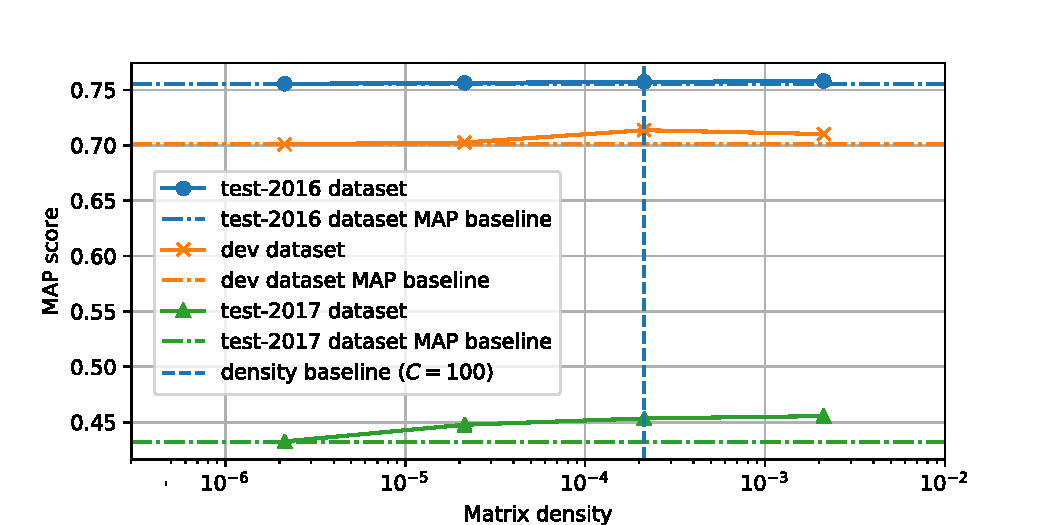
\includegraphics[trim={0.6cm 0.1cm 1.5cm 1.0cm}, scale=0.75]{figs/fig4}
\caption[A \abbr{MAP}-density plot for matrix $\mathbf S_{\textrm{lev}}$
and parameter $C$]{The \abbr{MAP}\index{map@\protect\abbr{MAP}}
  score plotted against the density of the matrix $\mathbf S_{\textrm{lev}}$
  \index{.slev@$\mathbf S_{\textrm{lev}}$} as we increase the parameter $C$
  \index{.c@$C$} from the value of $1$ (leftmost) to the value of $1{,}000$
  (rightmost). For every dataset, the baseline \abbr{MAP} score
  corresponds to using the cosine as a measure of similarity between two
  documents. Baseline density corresponds to the default value of~$C$.}
  \label{fig:similarity-fig4}
\end{figure}

\begin{figure}[p]
\centering%
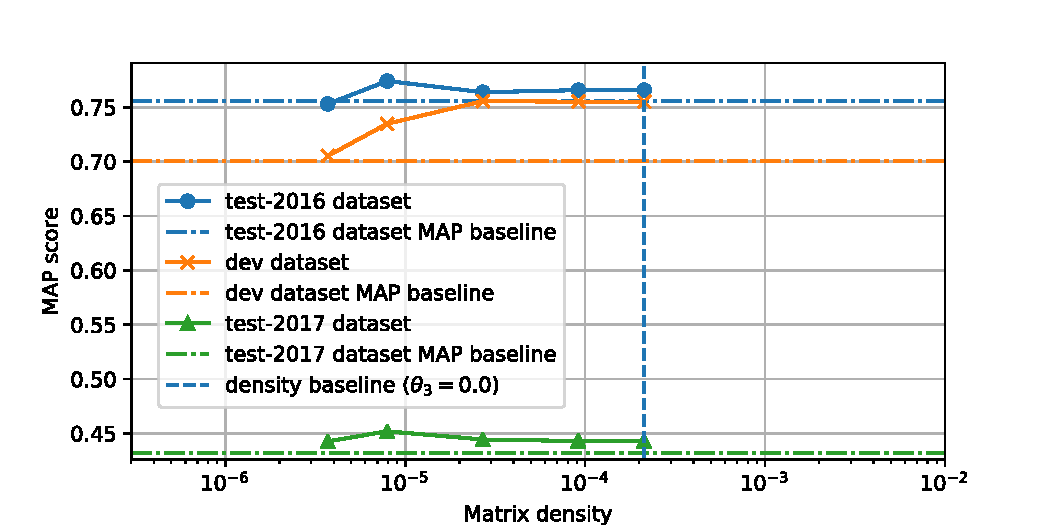
\includegraphics[trim={0.6cm 0.1cm 1.5cm 1.0cm}, scale=0.75]{figs/fig5}
\caption[A \abbr{MAP}-density plot for matrix $\mathbf S_{\textrm{lev}}$
and parameter $\theta_3$]{The
  \abbr{MAP}\index{map@\protect\abbr{MAP}} score plotted against the density of
  the matrix $\mathbf S_{\textrm{lev}}$ \index{.slev@$\mathbf S_{\textrm{lev}}$}
  as we increase the parameter $\theta_3$\index{.h3@$\theta_3$} from
  the value of $0.8$ (leftmost) to the value of $0$ (rightmost). For every
  dataset, the baseline \abbr{MAP} score corresponds to using the cosine as a measure
  of similarity between two documents. Baseline density corresponds to the
  default value~of~$\theta_3$.}
  \label{fig:similarity-fig5}
\end{figure}

\begin{figure}[p]
\centering%
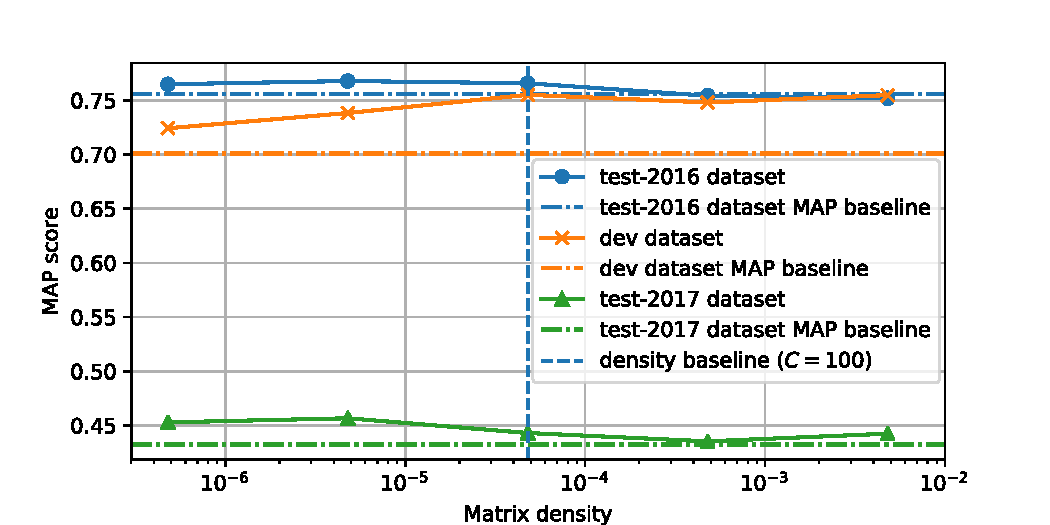
\includegraphics[trim={0.6cm 0.1cm 1.5cm 1.0cm}, scale=0.75]{figs/fig2}
\caption[A \abbr{MAP}-density plot for matrix $\mathbf S_{\textrm{rel}}$
and parameter $C$]{The \abbr{MAP}\index{map@\protect\abbr{MAP}}
  score plotted against the density of the matrix $\mathbf S_{\textrm{rel}}$
  \index{.srel@$\mathbf  S_{\textrm  {rel}}$} as we increase the parameter $C$
  \index{.c@$C$} from the value of $1$ (leftmost) to the value of $10{,}000$
  (rightmost). For every dataset, the baseline \abbr{MAP} score
  corresponds to using the cosine as a measure of similarity between two
  documents. Baseline density corresponds to the default value~of~$C$.}
  \label{fig:similarity-fig2}
\end{figure}

\begin{figure}[p]
\centering%
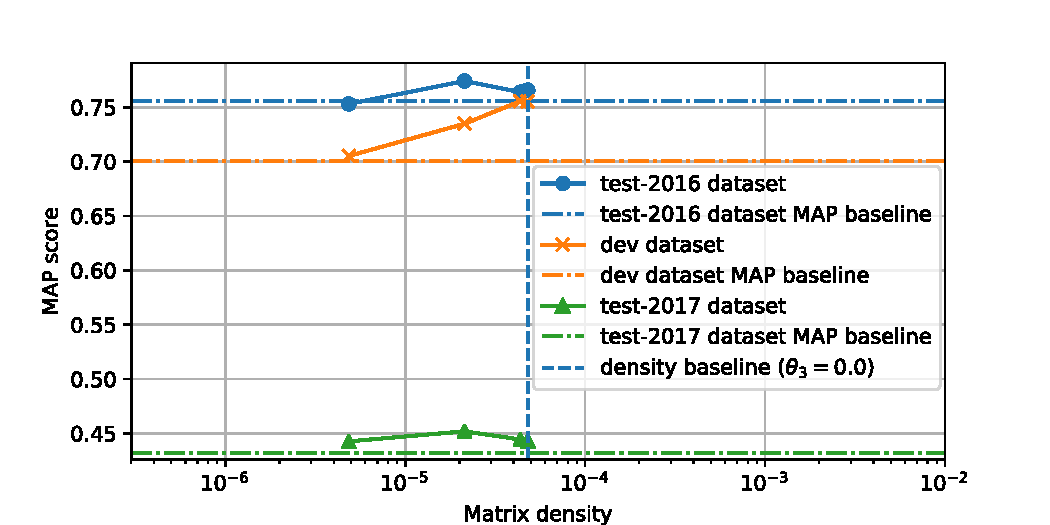
\includegraphics[trim={0.6cm 0.1cm 1.5cm 1.0cm}, scale=0.75]{figs/fig3}
\caption[A \abbr{MAP}-density plot for matrix $\mathbf S_{\textrm{rel}}$
and parameter $\theta_3$]{The
  \abbr{MAP}\index{map@\protect\abbr{MAP}} score plotted against the density of
  the matrix $\mathbf S_{\textrm{rel}}$ \index{.srel@$\mathbf S_{\textrm{rel}}$}
  as we increase the parameter $\theta_3$\index{.h3@$\theta_3$} from
  the value of $0.8$ (leftmost) to the value of $0.2$ (rightmost). For every
  dataset, the baseline \abbr{MAP} score corresponds to using the cosine as a measure
  of similarity between two documents. Baseline density corresponds to the
  default value~of~$\theta_3$.}
  \label{fig:similarity-fig3}
\end{figure}

\begin{figure}[tb]
\centering%
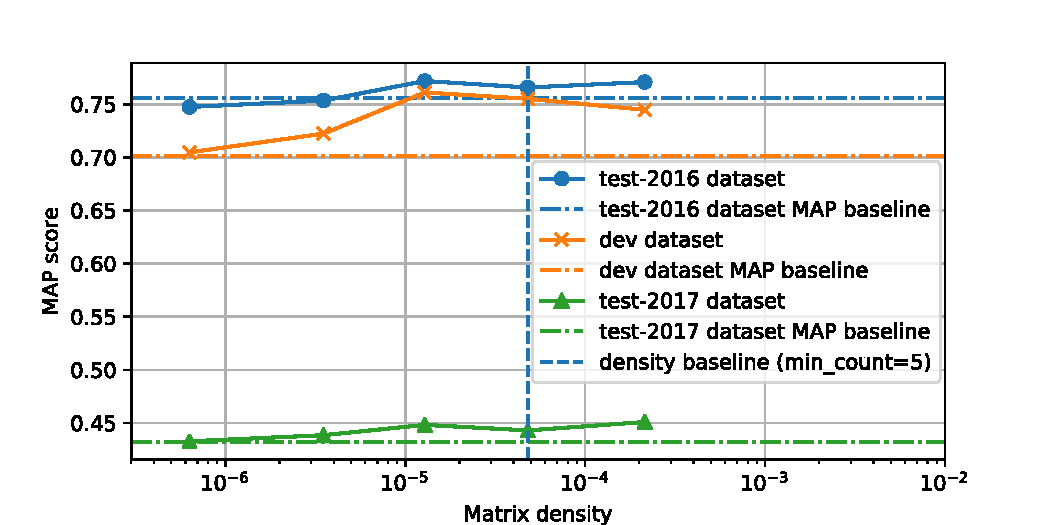
\includegraphics[trim={0.6cm 0.1cm 1.5cm 1.0cm}, scale=0.75]{figs/fig1}
\caption[A \abbr{MAP}-density plot for matrix $\mathbf S_{\textrm{rel}}$
and parameter \texttt{min\_count}]{The
  \abbr{MAP}\index{map@\protect\abbr{MAP}} score plotted against the density of
  the matrix $\mathbf S_{\textrm{rel}}$\index{.srel@$\mathbf S_{\textrm{rel}}$}
  as we increase the parameter
  \texttt{min\_count}\index{.mincount@\texttt{min\_count}} from the value of
  $5{,}000$ (leftmost) to the value of $0$ (rightmost). For every
  dataset, the baseline \abbr{MAP} score corresponds to using the cosine as a
  measure of similarity between two documents. Baseline density corresponds to
  the default value of \texttt{min\_count}.}
  \label{fig:similarity-fig1}
\end{figure}

\section{Results}
\label{sec:similarity-results}
By looking at \abbr{MAP}\index{map@\abbr {MAP}}-density plots of matrices
$\mathbf S_{\textrm{lev}}$ and $\mathbf S_{\textrm{rel}}$
\index{.slev@$\mathbf  S_{\textrm  {lev}}$}
\index{.srel@$\mathbf  S_{\textrm  {rel}}$}
in figures~\ref{fig:similarity-fig4}--\ref{fig:similarity-fig1},
several patterns emerge. Adjusting the parameter $C$\index{.c@$C$} leads to
higher \abbr{MAP} scores that adjusting the parameter
$\theta_3$\index{.h3@$\theta _3$} does. Increasing the density of $\mathbf
S$\index{.s@$\mathbf S$} leads to small or no increase in \abbr{MAP}, which
suggests that the extended model\index{standard model!extended} quickly reaches
a saturation point after which additional density of $\mathbf S$ does not lead
to an improvement in quality.

Looking at the individual figures, Figure~\ref{fig:similarity-fig5} shows that
with the matrix $\mathbf S_{\textrm{lev}}$, the
elements with a value of $s_{ij}$ below $0.4$ are of limited usefulness to the model.
Reintroducing these elements increases the density, but leads to no improvement
in the \abbr{MAP} score as evidenced by the flat right tails of the plotted
line segments.
Figure~\ref{fig:similarity-fig2} shows that the subtask~B dev and test datasets behave
very differently with respect to the parameter $C$\index{.c@$C$} for the
matrix $\mathbf S_{\textrm{rel}}$. Whereas the test datasets seem to benefit
from the sparsification of $\mathbf S$, the dev dataset follows a reverse trend
and consistently benefits from the increased density of $\mathbf S$.
Figure~\ref{fig:similarity-fig3} shows that with the matrix
$\mathbf S_{\textrm{rel}}$, all $C=100$ nearest neighbors $j$ of each term $i$
receive a value of $s_{ij}$ above $0.2$ and lower values of the parameter $\theta_3$
are therefore ineffective in further increasing the density of $\mathbf
S$\index{.s@$\mathbf S$}.
\index{.slev@$\mathbf  S_{\textrm  {lev}}$}
\index{.srel@$\mathbf  S_{\textrm  {rel}}$}

Considering the results in tables~\ref{tab:similarity-results-2016} and
\ref{tab:similarity-results-2017}, the highest rank across both subtask~B test datasets
was achieved by the ensemble matrix $\mathbf S_{\avg}$\index{.savg@$\mathbf
S_{\avg}$}. The matrices $\mathbf S_{\textrm{lev}}$ and
$\mathbf S_{\textrm{rel}}$\index{.slev@$\mathbf  S_{\textrm  {lev}}$}
\index{.srel@$\mathbf  S_{\textrm  {rel}}$} using default parameters
steadily outperformed the standard model.

The results for the models using soft cosine\index{cosine
similarity!soft} with hard normalization\index{normalization!hard} vary
wildly between the datasets; the most stable results were achieved with the
Google News Word2vec\index{Word2vec} term embedding\index{term embedding}
model, which stays within a $1.2$ \abbr{MAP}\index{map@\abbr {MAP}} score radius
around the matrices $\mathbf S_{\textrm{lev}}$ and $\mathbf
S_{\textrm{rel}}$\index{.slev@$\mathbf  S_{\textrm  {lev}}$}
\index{.srel@$\mathbf  S_{\textrm  {rel}}$} using default parameters. This
shows that the query expansion approach described in
Section~\ref{sec:similarity-inverted-index} is in general not inferior to
soft cosine similarity with soft normalization and can be used to implement
the extended model~\index{standard model!extended} in a way that allows us to
update $\mathbf S$\index{.s@$\mathbf S$} over time without reindexing the
document collection. Using just the inner product instead of soft cosine
similarity in the context of Section~\ref{sec:similarity-vector-db} shows
promise on the 2016 test dataset, but performs poorly in the 2017 test dataset.

\section{Conclusion and future work}
\label{sec:similarity-conclusion}
In this \ifthesis chapter\else paper\fi, I developed an extension to the
standard model\index{standard
model} for modeling synonymy and I showed that is outperforms the standard
model on the text similarity task in the context of \abbr{QA}. Importantly, I
also showed that, unlike other models such as \index{LSA@\abbr{LSA}}\abbr{LSA}, a close
approximation of the described model can be implemented in a way that allows us
to update $\mathbf S$\index{.s@$\mathbf S$} over time without reindexing the
document collection. I also developed several matrices that model different
facets of term similarity; this is in contrast to models such as \abbr{LSA},
which are confined to a single measure of similarity such as term
co-occurences\index{term co-occurence}.

The discussion in Section~\ref{sec:similarity-complexity} showed that little is
known about the density of the change-of-basis matrix \index{.e@$\mathbf E$}
and of the vectors that were cast to the orthonormal basis
$\bm\delta$\index{.d@$\bm\delta$}. In Section~\ref{sec:similarity-measures}, I
introduced the notion of supervised ensemble term similarity matrices, but no
concrete implementation was described and evaluated. These are both fruitful
venues for future work.

\FloatBarrier

\begin{sidewaystable}[p]
\pagestyle{empty}
\index{.srel@$\mathbf  S_{\textrm  {rel}}$}
\index{.slev@$\mathbf  S_{\textrm  {lev}}$}
\index{.savg@$\mathbf S_{\avg}$}
\index{.h3@$\theta _3$}
\index{.c@$C$}
\index{normalization!hard}
\index{normalization!soft}
\index{cosine similarity!soft}
\index{cosine similarity}
\centering
\begin{liningfigs}
\footnotesize
\begin{tabular}{llllrlrl}
Matrix $\mathbf S$ &
  Term embedding model &
  Normalization &
  Measure &
  $C$ &
  $\theta_3$ &
  \texttt{min\_count} &
  \abbr{MAP}\index{map@\abbr {MAP}} \\ \toprule
$\mathbf S_{\textrm{rel}}$ & w2v.ql & soft & soft cosine & $100$ & $0.6$ & $5$ & $77.41$ \\
$\mathbf S_{\textrm{rel}}$ & w2v.ql & soft & soft cosine & $100$ & $0$ & $50$ & $77.18$ \\
$\mathbf S_{\textrm{rel}}$ & w2v.ql & hard & soft cosine & $100$ & $0$ & $5$ & $77.10$ \\
$\mathbf S_{\textrm{rel}}$ & w2v.ql & soft & soft cosine & $100$ & $0$ & $0$ & $77.08$ \\
$\mathbf S_{\textrm{rel}}$ & w2v.ql & soft & soft cosine & $10$ & $0$ & $5$ & $76.78$ \\
\multicolumn{4}{l}{\bfseries SemEval-2016 task~3 subtask~B winner (\abbr{UH-PRHLT}-primary)} &
  --- &
  --- &
  --- &
  \bfseries76.70 \\
$\mathbf S_{\textrm{avg}}$ & w2v.ql & soft & soft cosine & $100$ & $0$ & $5$ & $76.61$ \\
$\mathbf S_{\textrm{rel}}$ & w2v.ql & soft & soft cosine & $100$ & $0.2$ & $5$ & $76.57$ \\
$\mathbf S_{\textrm{rel}}$ & w2v.ql & soft & soft cosine & $100$ & $0$ & $5$ & $76.57$ \\ % charlet
$\mathbf S_{\textrm{rel}}$ & w2v.ql & soft & soft cosine & $1$ & $0$ & $5$ & $76.48$ \\
$\mathbf S_{\textrm{rel}}$ & w2v.ql & soft & soft cosine & $100$ & $0.4$ & $5$ & $76.38$ \\
$\mathbf S_{\textrm{lev}}$ & --- & soft & soft cosine & $100$ & $0.4$ & --- & $75.88$ \\
$\mathbf S_{\textrm{lev}}$ & --- & soft & soft cosine & $100$ & $0.6$ & --- & $75.81$ \\
$\mathbf S_{\textrm{lev}}$ & --- & soft & soft cosine & $1000$ & $0$ & --- & $75.80$ \\
$\mathbf S_{\textrm{rel}}$ & w2v.ql & --- & inner product & $100$ & $0$ & $5$ & $75.79$ \\
$\mathbf S_{\textrm{lev}}$ & --- & soft & soft cosine & $100$ & $0.2$ & --- & $75.72$ \\
$\mathbf S_{\textrm{lev}}$ & --- & soft & soft cosine & $100$ & $0$ & --- & $75.72$ \\
$\mathbf S_{\textrm{lev}}$ & --- & soft & soft cosine & $100$ & $0.8$ & --- & $75.67$ \\
$\mathbf S_{\textrm{rel}}$ & w2v.googlenews & hard & soft cosine & $100$ & $0$ & $5$ & $75.64$ \\
$\mathbf S_{\textrm{lev}}$ & --- & soft & soft cosine & $10$ & $0$ & --- & $75.63$ \\
$\mathbf S_{\textrm{lev}}$ & --- & soft & soft cosine & $1$ & $0$ & --- & $75.55$ \\
--- & --- & --- & \bfseries cosine & --- & --- & --- & \bfseries 75.55 \\
$\mathbf S_{\textrm{rel}}$ & w2v.ql & soft & soft cosine & $1000$ & $0$ & $5$ & $75.42$ \\
$\mathbf S_{\textrm{rel}}$ & glove.common\_crawl & hard & soft cosine & $100$ & $0$ & $5$ & $75.42$ \\
$\mathbf S_{\textrm{rel}}$ & w2v.ql & soft & soft cosine & $100$ & $0$ & $500$ & $75.34$ \\
$\mathbf S_{\textrm{rel}}$ & w2v.ql & soft & soft cosine & $100$ & $0.8$ & $5$ & $75.30$ \\
$\mathbf S_{\textrm{rel}}$ & w2v.ql & soft & soft cosine & $10000$ & $0$ & $5$ & $75.19$ \\
\multicolumn{3}{l}{\bfseries SemEval-2016 task~3 subtask~B \abbr{IR}\index{ir@\protect\abbr{IR}} baseline} &
  --- &
  --- &
  --- &
  --- &
  \bfseries74.75 \\
$\mathbf S_{\textrm{rel}}$ & w2v.ql & soft & soft cosine & $100$ & $0$ & $5000$ & $74.74$ \\
$\mathbf S_{\textrm{rel}}$ & fasttext.enwiki & hard & soft cosine & $100$ & $0$ & $5$ & $74.73$ \\
$\mathbf S_{\textrm{rel}}$ & glove.enwiki\_gigaword5 & hard & soft cosine & $100$ & $0$ & $5$ & $72.78$ \\
\end{tabular}
\end{liningfigs}
\caption[Results for all configurations on the SemEval-2016 task~3
subtask~B test dataset]{%
  Results for all configurations on the 2016 subtask~B test dataset.
  Baselines are highlighted~in~bold.}
\label{tab:similarity-results-2016}
\end{sidewaystable}

\begin{sidewaystable}[p]
\pagestyle{empty}
\index{.srel@$\mathbf  S_{\textrm  {rel}}$}
\index{.slev@$\mathbf  S_{\textrm  {lev}}$}
\index{.savg@$\mathbf S_{\avg}$}
\index{normalization!hard}
\index{normalization!soft}
\index{cosine similarity!soft}
\index{cosine similarity}
\index{.h3@$\theta _3$}
\index{.c@$C$}
\centering
\begin{liningfigs}
\footnotesize
\begin{tabular}{llllrlrl}
Matrix $\mathbf S$ &
  Term embedding model &
  Normalization &
  Measure &
  $C$ &
  $\theta_3$ &
  \texttt{min\_count} &
  \abbr{MAP}\index{map@\abbr {MAP}} \\ \toprule
\multicolumn{4}{l}{\bfseries SemEval-2017 task~3 subtask~B winner (SimBow-primary)} &
  --- &
  --- &
  --- &
  \bfseries47.22 \\
$\mathbf S_{\textrm{avg}}$ & w2v.ql & soft & soft cosine & $100$ & $0$ & $5$ & $46.04$ \\
$\mathbf S_{\textrm{rel}}$ & w2v.ql & soft & soft cosine & $10$ & $0$ & $5$ & $45.67$ \\
$\mathbf S_{\textrm{lev}}$ & --- & soft & soft cosine & $1000$ & $0$ & --- & $45.55$ \\
$\mathbf S_{\textrm{rel}}$ & glove.common\_crawl & hard & soft cosine & $100$ & $0$ & $5$ & $45.49$ \\
$\mathbf S_{\textrm{lev}}$ & --- & soft & soft cosine & $100$ & $0.6$ & --- & $45.35$ \\
$\mathbf S_{\textrm{lev}}$ & --- & soft & soft cosine & $100$ & $0.0$ & --- & $45.34$ \\
$\mathbf S_{\textrm{lev}}$ & --- & soft & soft cosine & $100$ & $0.2$ & --- & $45.31$ \\
$\mathbf S_{\textrm{rel}}$ & w2v.ql & soft & soft cosine & $1$ & $0$ & $5$ & $45.29$ \\
$\mathbf S_{\textrm{lev}}$ & --- & soft & soft cosine & $100$ & $0.4$ & --- & $45.22$ \\
$\mathbf S_{\textrm{rel}}$ & w2v.ql & soft & soft cosine & $100$ & $0.6$ & $5$ & $45.20$ \\
$\mathbf S_{\textrm{rel}}$ & glove.enwiki\_gigaword5 & hard & soft cosine & $100$ & $0$ & $5$ & $45.13$ \\
$\mathbf S_{\textrm{rel}}$ & w2v.ql & soft & soft cosine & $100$ & $0$ & $0$ & $45.10$ \\
$\mathbf S_{\textrm{rel}}$ & fasttext.enwiki & hard & soft cosine & $100$ & $0$ & $5$ & $44.94$ \\
$\mathbf S_{\textrm{rel}}$ & w2v.ql & soft & soft cosine & $100$ & $0$ & $50$ & $44.83$ \\
$\mathbf S_{\textrm{lev}}$ & --- & soft & soft cosine & $10$ & $0$ & --- & $44.77$ \\
$\mathbf S_{\textrm{lev}}$ & --- & soft & soft cosine & $100$ & $0.8$ & --- & $44.65$ \\
$\mathbf S_{\textrm{rel}}$ & w2v.ql & soft & soft cosine & $100$ & $0.4$ & $5$ & $44.45$ \\
$\mathbf S_{\textrm{rel}}$ & w2v.ql & soft & soft cosine & $100$ & $0.2$ & $5$ & $44.31$ \\
$\mathbf S_{\textrm{rel}}$ & w2v.ql & soft & soft cosine & $100$ & $0$ & $5$ & $44.31$ \\
$\mathbf S_{\textrm{rel}}$ & w2v.ql & soft & soft cosine & $100$ & $0.8$ & $5$ & $44.28$ \\
$\mathbf S_{\textrm{rel}}$ & w2v.ql & soft & soft cosine & $10000$ & $0$ & $5$ & $44.25$ \\
$\mathbf S_{\textrm{rel}}$ & w2v.googlenews & hard & soft cosine & $100$ & $0$ & $5$ & $44.13$ \\
$\mathbf S_{\textrm{rel}}$ & w2v.ql & soft & soft cosine & $100$ & $0$ & $500$ & $43.86$ \\
$\mathbf S_{\textrm{rel}}$ & w2v.ql & hard & soft cosine & $100$ & $0$ & $5$ & $43.76$ \\
$\mathbf S_{\textrm{rel}}$ & w2v.ql & soft & soft cosine & $1000$ & $0$ & $5$ & $43.54$ \\
$\mathbf S_{\textrm{rel}}$ & w2v.ql & soft & soft cosine & $100$ & $0$ & $5000$ & $43.28$ \\
$\mathbf S_{\textrm{lev}}$ & --- & soft & soft cosine & $1$ & $0$ & --- & $43.27$ \\
--- & --- & --- & \bfseries cosine & --- & --- & --- & \bfseries 43.25 \\
$\mathbf S_{\textrm{rel}}$ & w2v.ql & --- & inner product & $100$ & $0$ & $5$ & $42.17$ \\
\multicolumn{3}{l}{\bfseries SemEval-2017 task~3 subtask~B \abbr{IR}\index{ir@\protect\abbr{IR}} baseline} &
  --- &
  --- &
  --- &
  --- &
  \bfseries41.85 \\
\end{tabular}
\end{liningfigs}
\caption[Results for all configurations on the SemEval-2017 task~3
subtask~B test dataset]{%
  Results for all configurations on the 2017 subtask~B test dataset.
  Baselines are highlighted~in~bold.}
\label{tab:similarity-results-2017}
\end{sidewaystable}

\ifreview\else
\subsection*{Acknowledgments}
\abbr{\noexpand\MakeUppercase TAČR} Omega grant \abbr{TD03000295} is gratefully acknowledged.
\fi

%% The following section corresponds to the bibliography:
\nocite{ir:Zezula2006} %% The recommended literature.
\nocite{ml:IntroIR2008}
\nocite{mikolov2013efficient}
\begingroup\sloppy
\printbibliography[heading=bibintoc]
\endgroup

\end{document}
